\documentclass{beamer}

\usepackage{graphicx}
\usepackage{multimedia}
\usepackage{amsmath}
\usepackage{amsfonts}
\usepackage{tikz}
\usetikzlibrary{arrows.meta, decorations.pathreplacing, matrix}

\usepackage[style=authoryear, backend=biber, maxbibnames=99,
            maxcitenames=2, giveninits=true, url=false, isbn=false]{biblatex}
\addbibresource{lab-meeting.bib}

% Source citation pinned to the bottom-right corner of a slide (for figures
% reproduced from other works). Usage: \figsource{\cite{key}}.
\newcommand{\figsource}[1]{%
    \begin{tikzpicture}[remember picture, overlay]
        \node[anchor=south east, font=\scriptsize, text=gray,
              inner sep=5pt] at (current page.south east) {Source: #1};
    \end{tikzpicture}%
}

% \usetheme{Madrid}

\setbeamersize{
    text margin left=0.5cm,
    text margin right=0.5cm
}

\title{Continuous Attractors in Retrosplenial Cortex}
\subtitle{Branco Lab Meeting}
\author{Jake Laherty}
\date{\today}

\begin{document}

\maketitle

\begin{frame}{Overview}
    
    \begin{itemize}
        \item<1-> Motivation
        \item<2-> Data analysis: are there continuous attractors in retrosplenial cortex?
        \begin{itemize}
            \item<3-> Probably but [caveats]...
        \end{itemize}
        \item<4-> Modelling: do continuous attractors arise in RNNs?
        \begin{itemize}
            \item<5-> Yes but [caveats]...
        \end{itemize}
        \item<6-> (Some) Theory of continuous attractors
        \item<7-> Next steps
        \begin{itemize}
            \item<8-> Theory
            \item<9-> Experiments
        \end{itemize}
    \end{itemize}

\end{frame}

\begin{frame}{Motivation}

    \centering
    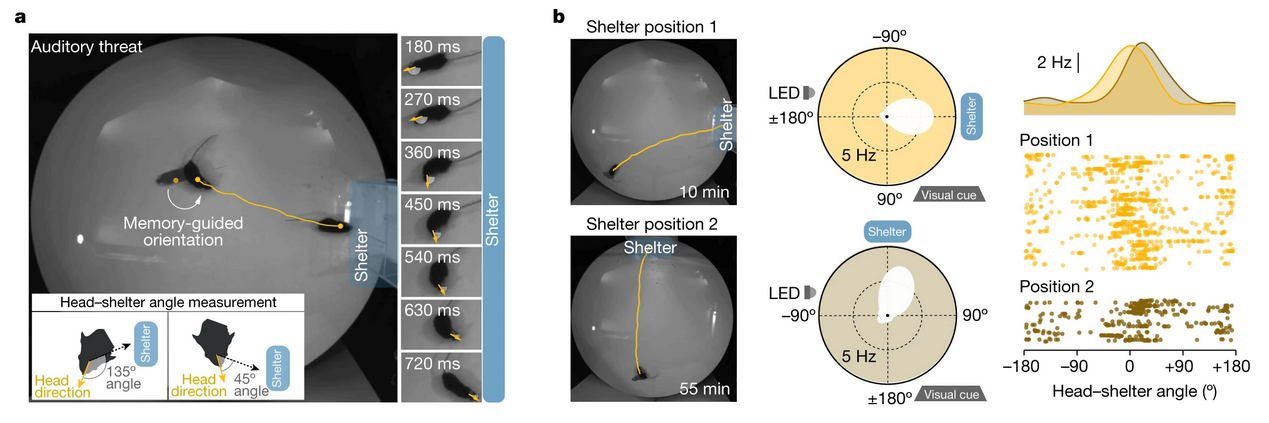
\includegraphics[width=0.9\textwidth]{presentation_figures/campagner_et_al_2022_f1.png}

    \figsource{\cite{campagner2022}}
\end{frame}

\begin{frame}{Motivation}

    \begin{itemize}
        \item<1-> Imagine you're a neural circuit, trying to keep track of some variable in the world, $\theta(t)$
        \item<2-> You need to be able to track small updates over time, $\frac{d}{dt} \theta(t)$ (and possibly allow hard resets)
        \item<3-> For example:
        \begin{itemize}
            \item<4-> Eye position \parencite{seung2000}
            \item<5-> Orientation tuning \parencite{benyishai1995}
            \item<6-> Position \parencite{burak2009}
            \item<7-> Task variables \parencite{perich2025,langdon2023}
        \end{itemize}
    \end{itemize}
    
    \uncover<8->{
        The canonical model for this situation is the continuous attractor:
        fixed points of a dynamical system correspond to particular values of $\theta$.
    }

\end{frame}



\begin{frame}{Motivation}

    What we were motivated by is coordinate transformations.

    Suppose we have two interacting continuous attractor circuits:
    \begin{itemize}
        \item They track variables $\theta_1(t)$ and $\theta_2(t)$ whose zero is given by an external landmark (e.g. head direction, position).
        \item We want to compute a new variable $\varphi(t) = f(\theta_1(t), \theta_2(t))$ (e.g. head-shelter angle).
    \end{itemize}
    
    The canonical model for this is to form an intermediate circuit tuned to combinations of $\theta_1$ and $\theta_2$ as a basis for $f$; e.g. \textcite{bicanski2016}:

    \centering
    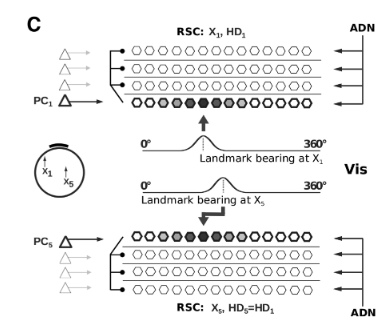
\includegraphics[width=0.4\textwidth]{presentation_figures/bicanski_burgess_2016_f1.png}

    \figsource{\cite{bicanski2016}}
\end{frame}




{
\setbeamertemplate{navigation symbols}{}
\begin{frame}[plain]
    \centering
    \vfill

    {\usebeamerfont{title}\usebeamercolor[fg]{title}
    \Huge Data Analysis\par}

    \vspace{0.8em}

    {\usebeamerfont{subtitle}\usebeamercolor[fg]{subtitle}
    \Large Are there continuous attractors in retrosplenial cortex?\par}

    (NB: all data generously supplied by Jasmine Reggiani)

    \vfill
\end{frame}
}

\begin{frame}
    \centering
    \movie[
        width=0.9\textwidth,
        showcontrols
    ]{
        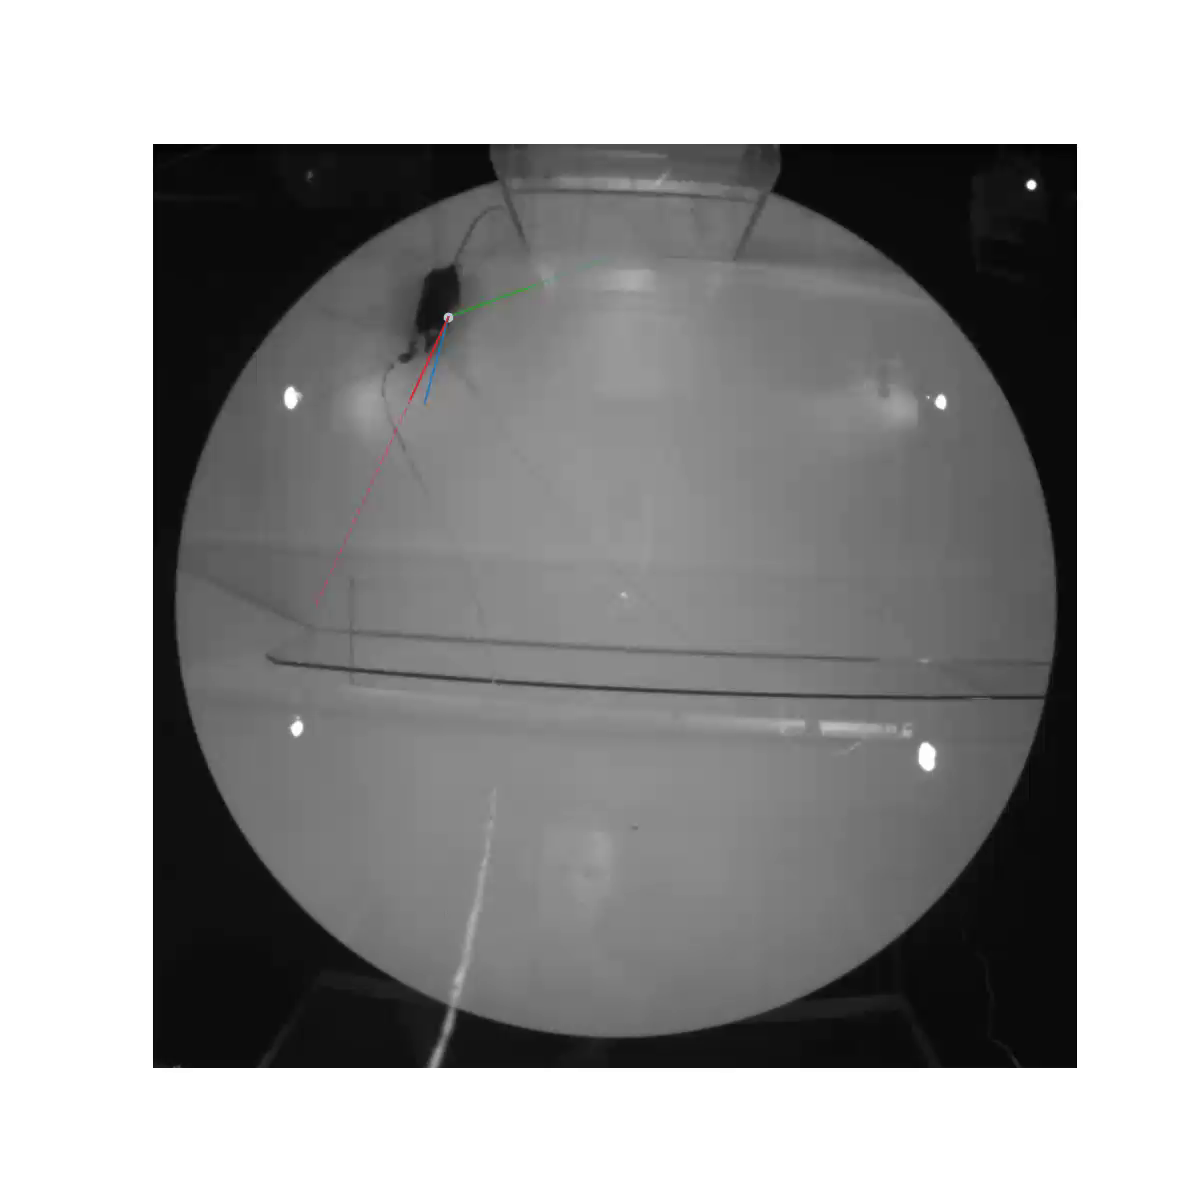
\includegraphics[width=0.9\textwidth]{presentation_figures/0_preview.png}
    }{0_cam_overlay.mp4}
\end{frame}

\begin{frame}
    \begin{itemize}
        \item Mice (here 3 animals, 12 sessions total) explore arena with a shelter and a barrier open at one side.
        \item Halfway through the session, the barrier opening is flipped to the other side.
        \item Neurons in retrosplenial cortex are recorded with Neuropixels ($N=2075$ single units).
        \item Here we consider periods of free exploration (no escaping, no homing)
        \item We track: head-direction and barrier-direction (angles relative to left-center of frame); head-shelter angle and head-barrier angle (angles relative to head-direction)
    \end{itemize}
\end{frame}

\begin{frame}
    \centering
    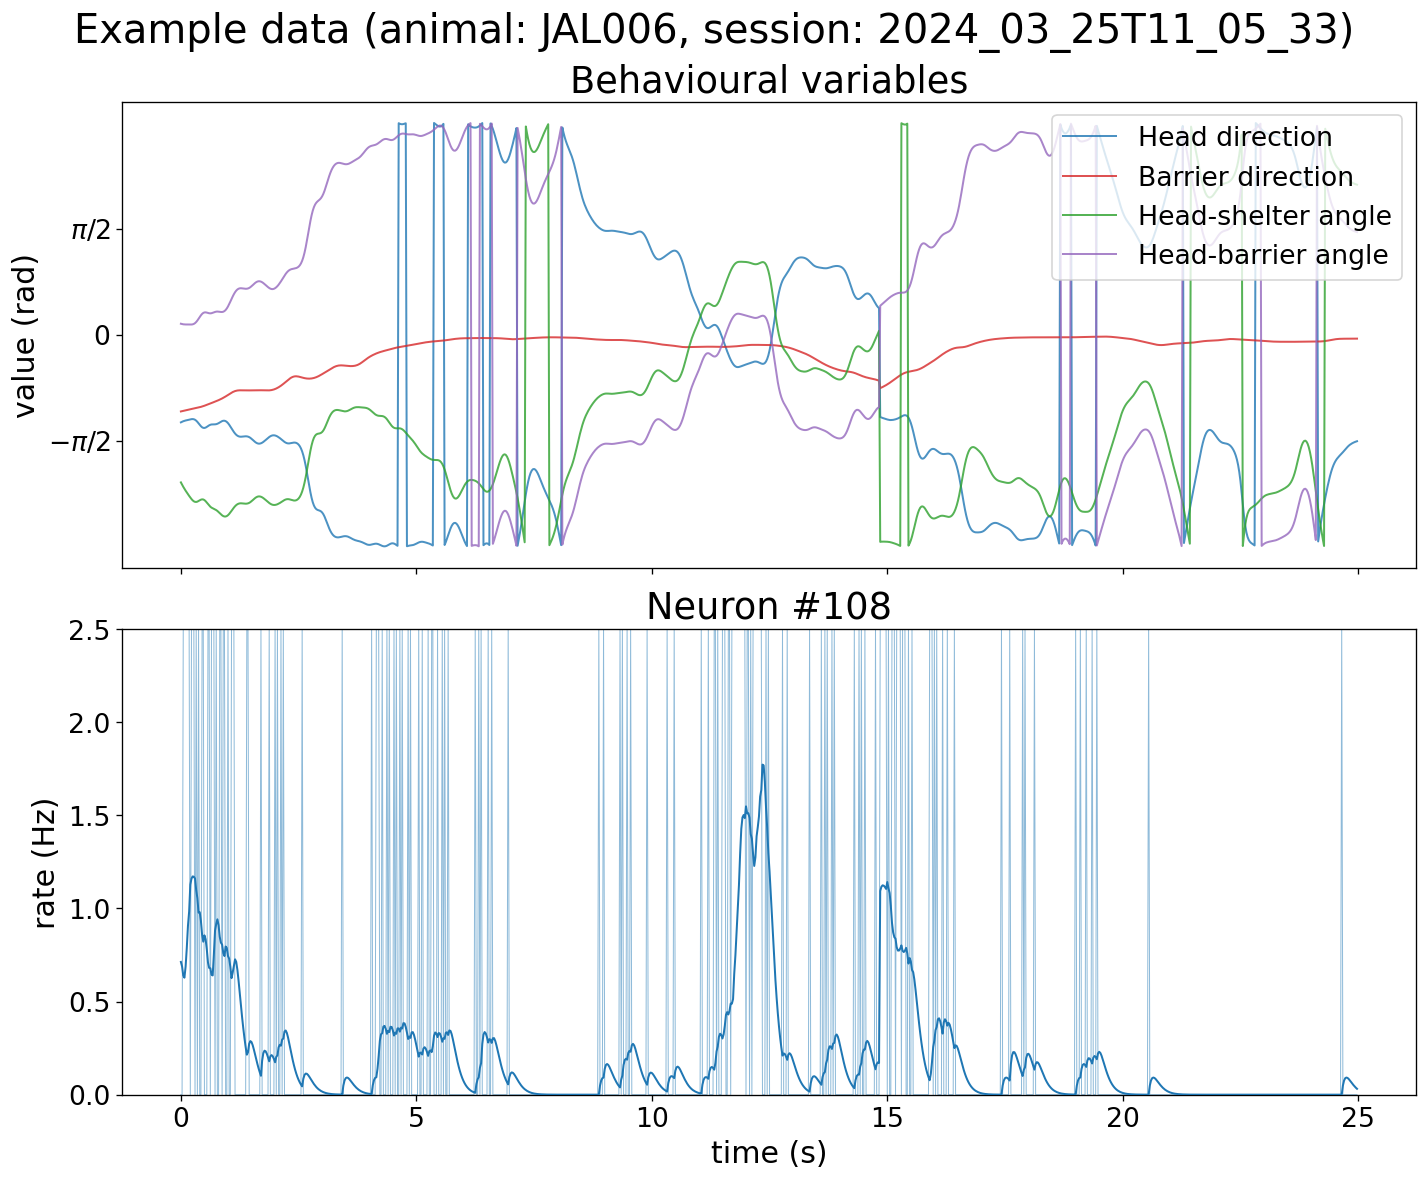
\includegraphics[width=0.9\textwidth]{presentation_figures/item1_timeseries.png}
\end{frame}

\begin{frame}{Tuning analysis}
    
    In what follows, we will be looking at tuning curves (drawing significantly from \textcite{clark2025}). These are computed by:

    \begin{itemize}
        \item Partitioning sessions into $K$ disjoint, contiguous periods (here $K=2$).
        \item Binning each behavioural variable into $D=100$ bins and computing the average firing rate of each neuron in each bin.
        \item Fitting a curve to these emprical within-partition tuning curves using a periodic Gaussian Process.
        \item Choosing the parameters of this GP (kernel length and amplitude scales) by maximising the cross-partition Poisson likelihood.
        \item Fitting a curve to the whole session using the average cross-validated parameters across all partitions.
    \end{itemize}
    
\end{frame}

\begin{frame}
    \centering
    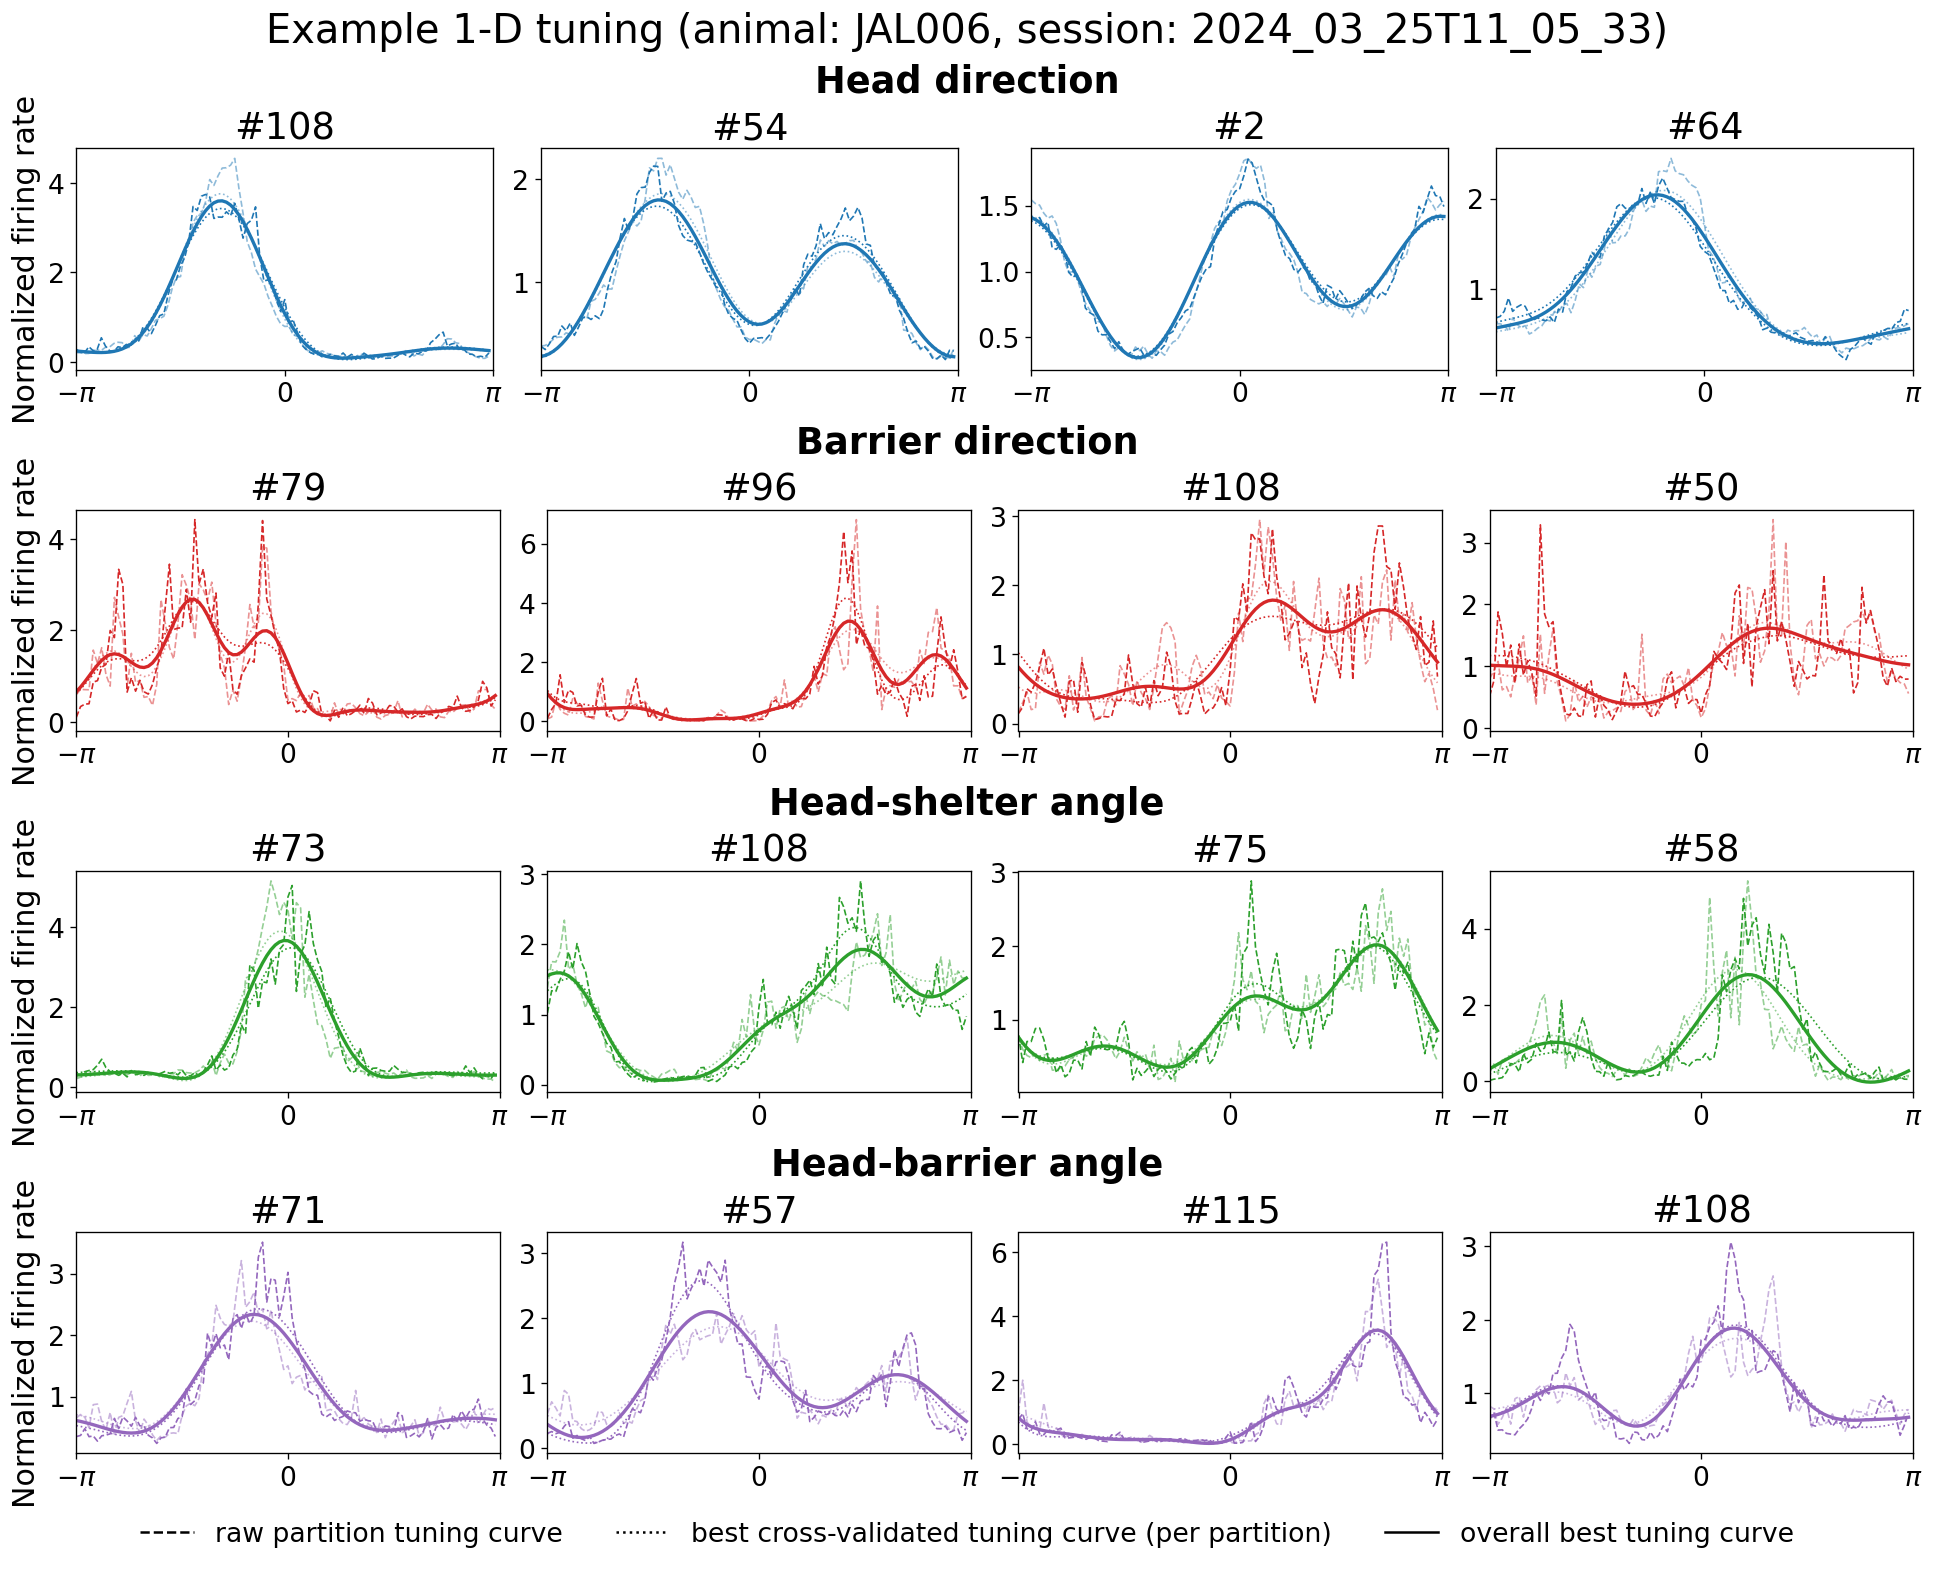
\includegraphics[width=0.9\textwidth]{presentation_figures/item2_tuning.png}
\end{frame}

\begin{frame}
    \centering
    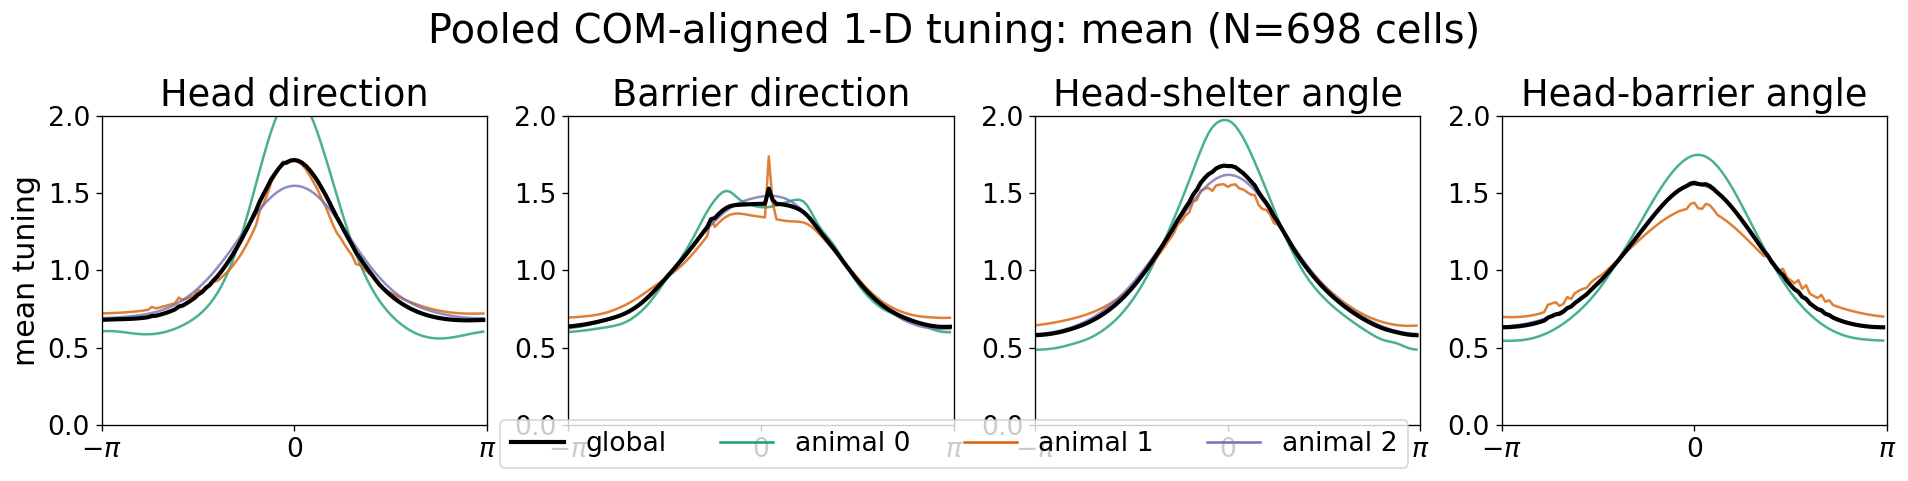
\includegraphics[width=0.9\textwidth]{presentation_figures/item3_pooled_mean.png}\
    \vfill
    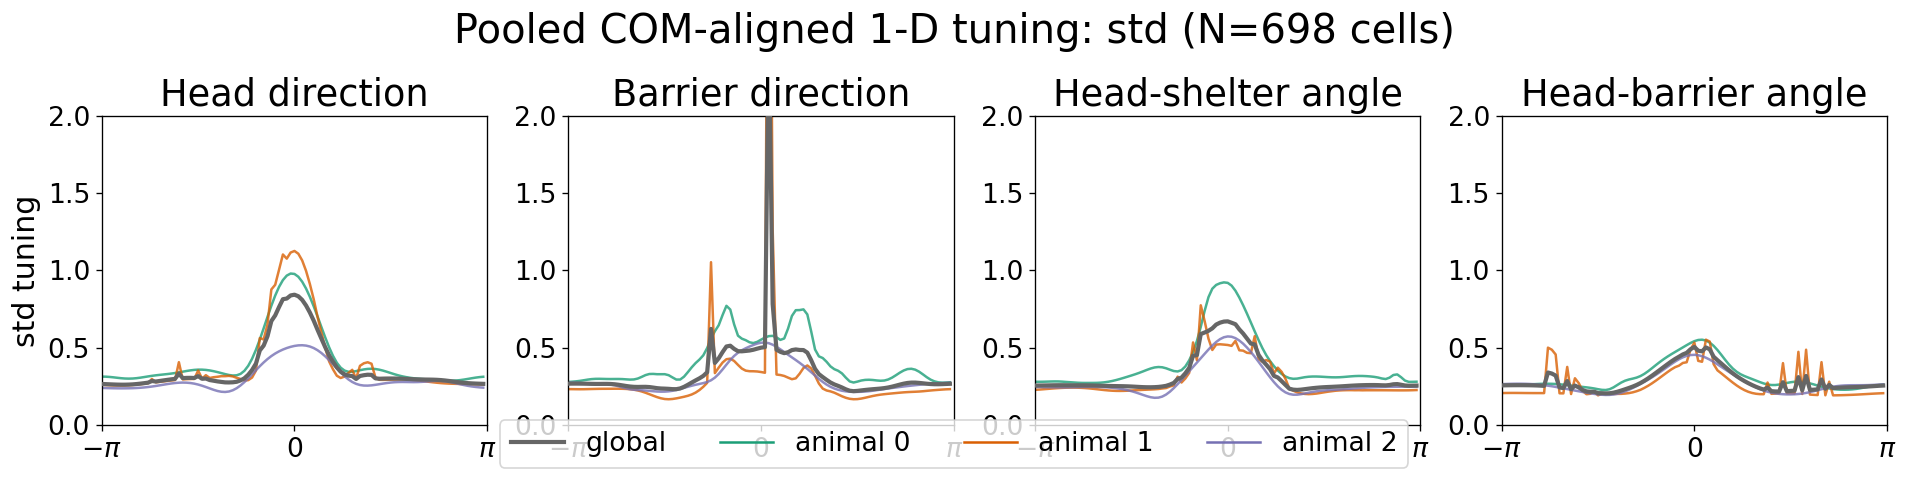
\includegraphics[width=0.9\textwidth]{presentation_figures/item3_pooled_std.png}
    \vfill
\end{frame}

\begin{frame}{Tuning Analysis}
    What does this tell us?

    \begin{itemize}
        \item Individual neurons can be described by tuning to behavioural variables.
        \item Across the population, the shape of these tuning curves is heterogeneous.
    \end{itemize}

    We can model this situation as a finite sample of neurons in 4 separate continuous attractor networks with disordered embeddings.

\end{frame}

\begin{frame}
    Consider the correlation matrix of tuning curves:

    \begin{equation*}
        C^{\phi}(\theta, \theta') = \frac{1}{N} \sum_i^N \phi^*_i(\theta) \phi^*_i(\theta')
    \end{equation*}

    where $\phi^*_i(\theta)$ is the firing rate of neuron $i$ as a function of the tracked variable $\theta$ (i.e. its tuning curve)

    \centering
    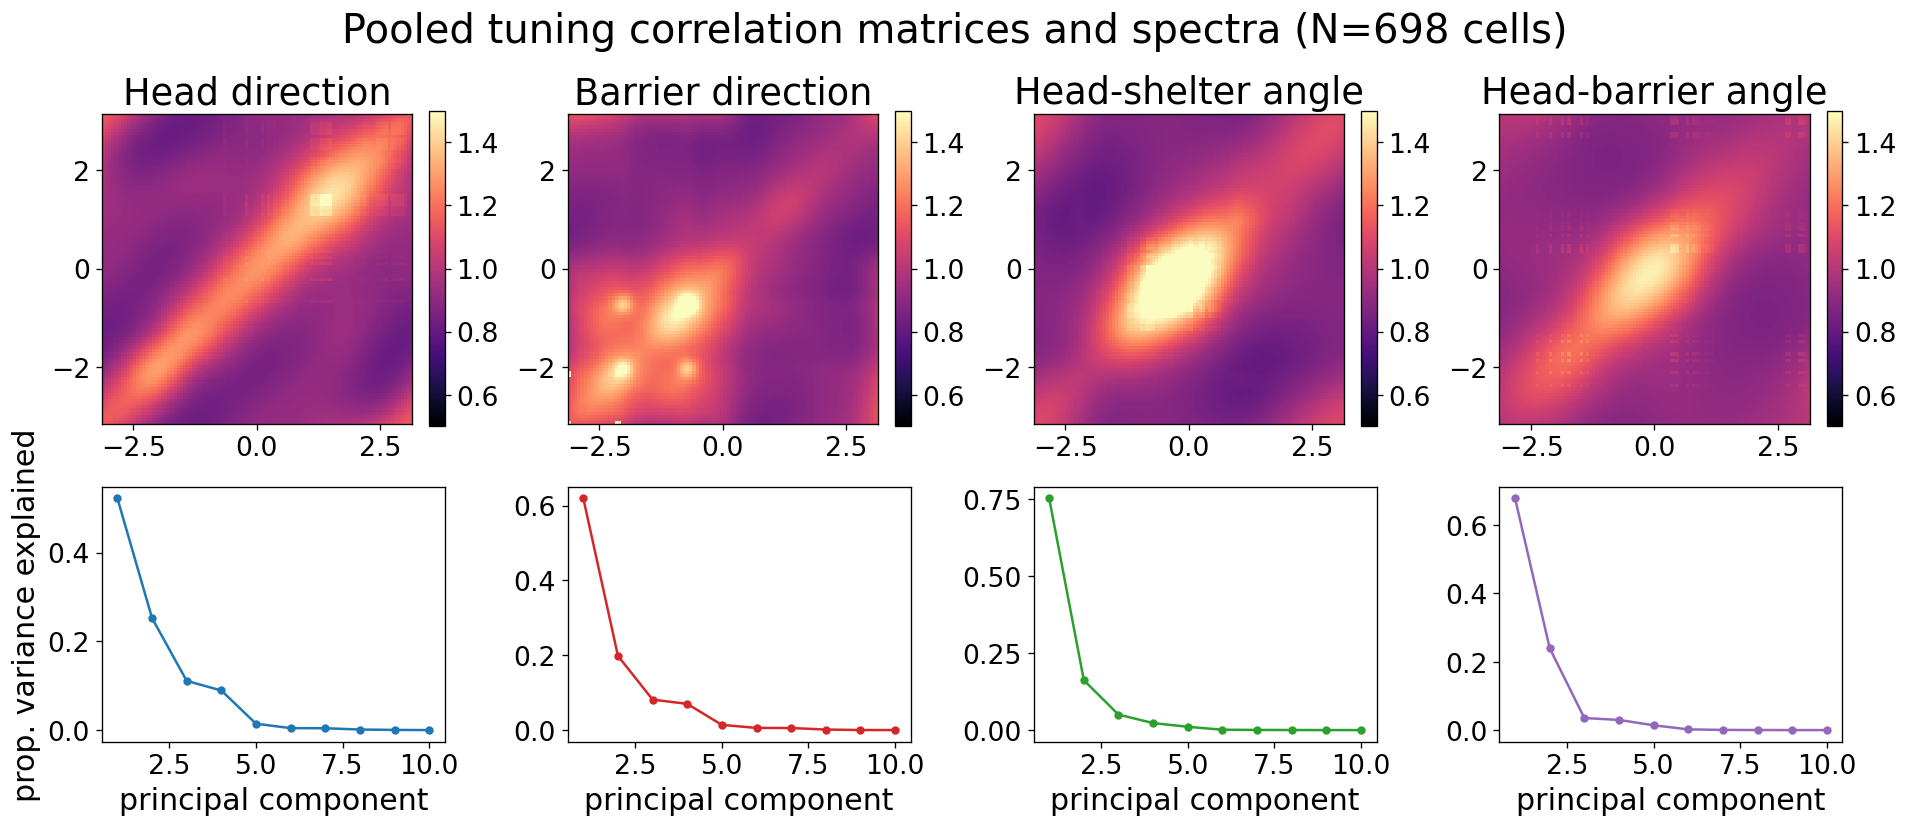
\includegraphics[width=0.9\textwidth]{presentation_figures/item7_corr.png}
\end{frame}

\begin{frame}{Tuning Analysis: Generative Model}
    We can construct a generative model of tuning curves as follows:

    \begin{equation*}
        \phi^*(\theta) = f(x^*(\theta))
    \end{equation*}

    for some non-linear activation function $f$ and the tuning curve of 'somatic voltage' $x^*(\theta)$. We parametrise these as:

    \begin{equation*}
        x^*(\theta) \sim \mathcal{GP}(0, \Gamma(\theta - \theta'; \sigma)) 
    \end{equation*}

    \begin{equation*}
        f(x) = \frac{1}{Z[x]} \log \left( 1 + e^{\beta(x - b)} \right)
    \end{equation*}

    We fit the hyperparameters $(\sigma, \beta, b)$ by minimising MSE between tuning correlation matrices sampled from the generative process and the empirical ones.
    
\end{frame}

\begin{frame}
    \begin{center}
        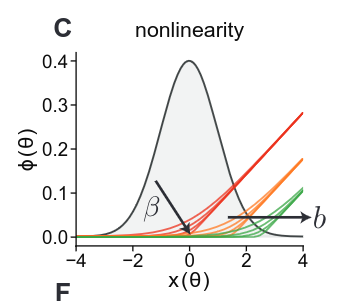
\includegraphics[width=0.75\textwidth]{presentation_figures/clark_et_al_2025_f5.png}
    \end{center}

    \figsource{\cite{clark2025}}
\end{frame}

\begin{frame}
    \centering
    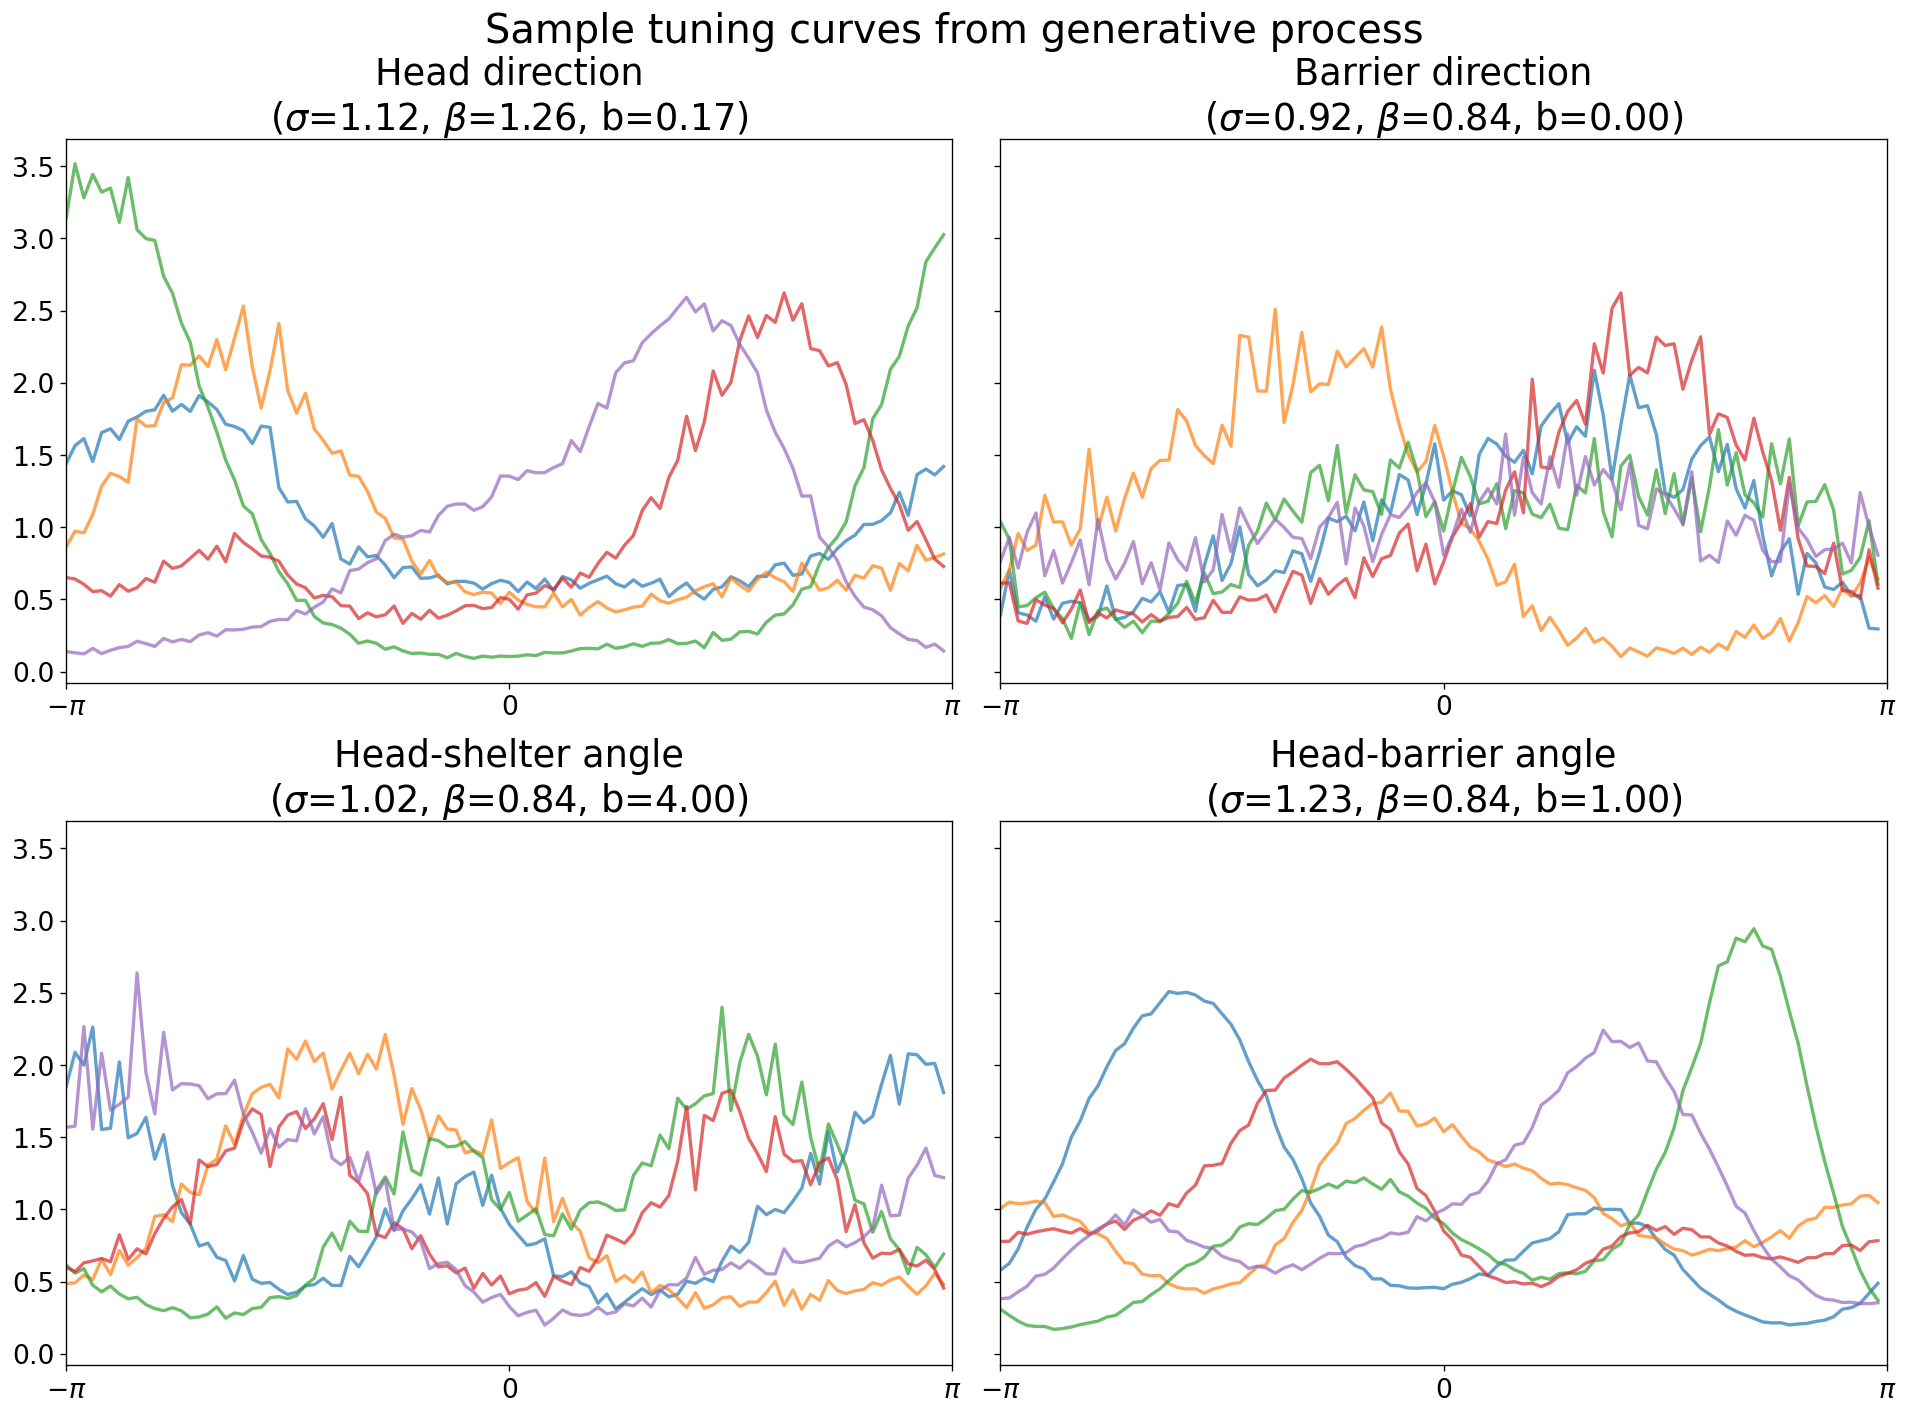
\includegraphics[width=0.9\textwidth]{presentation_figures/item8_generative_draws.png}
\end{frame}

\begin{frame}
    \centering
    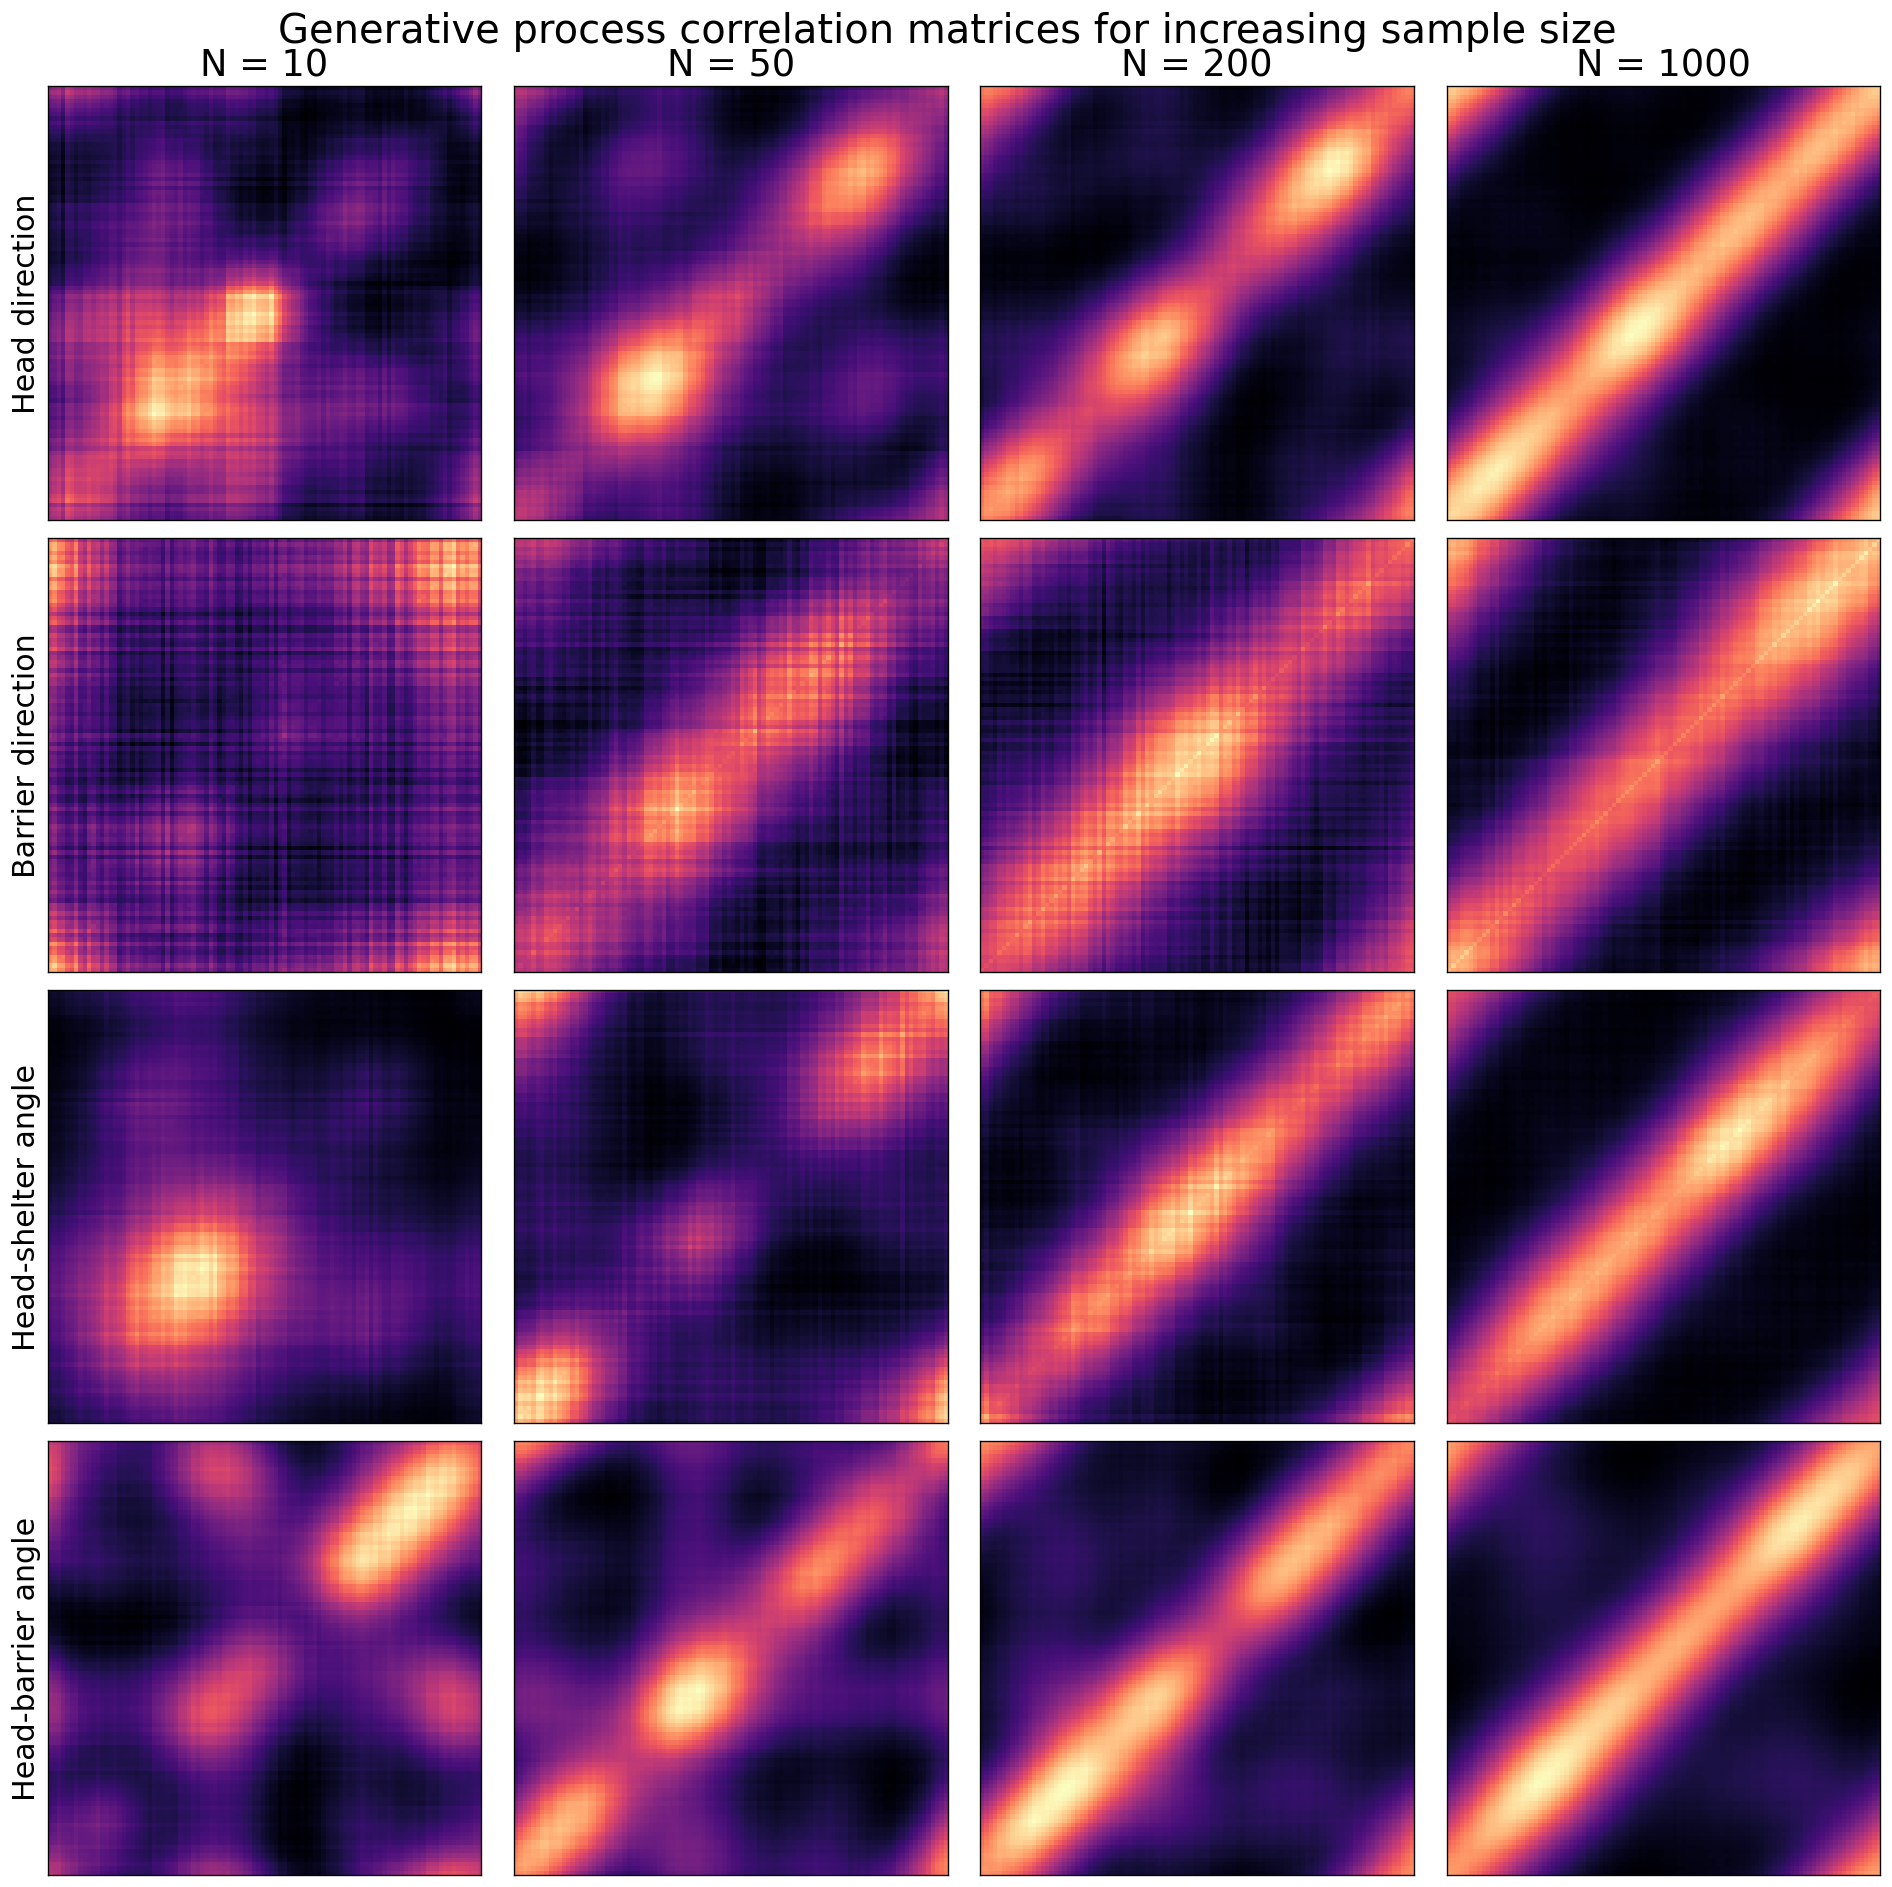
\includegraphics[width=0.7\textwidth]{presentation_figures/item9_corr_vs_samples.png}
\end{frame}

\begin{frame}
    \centering
    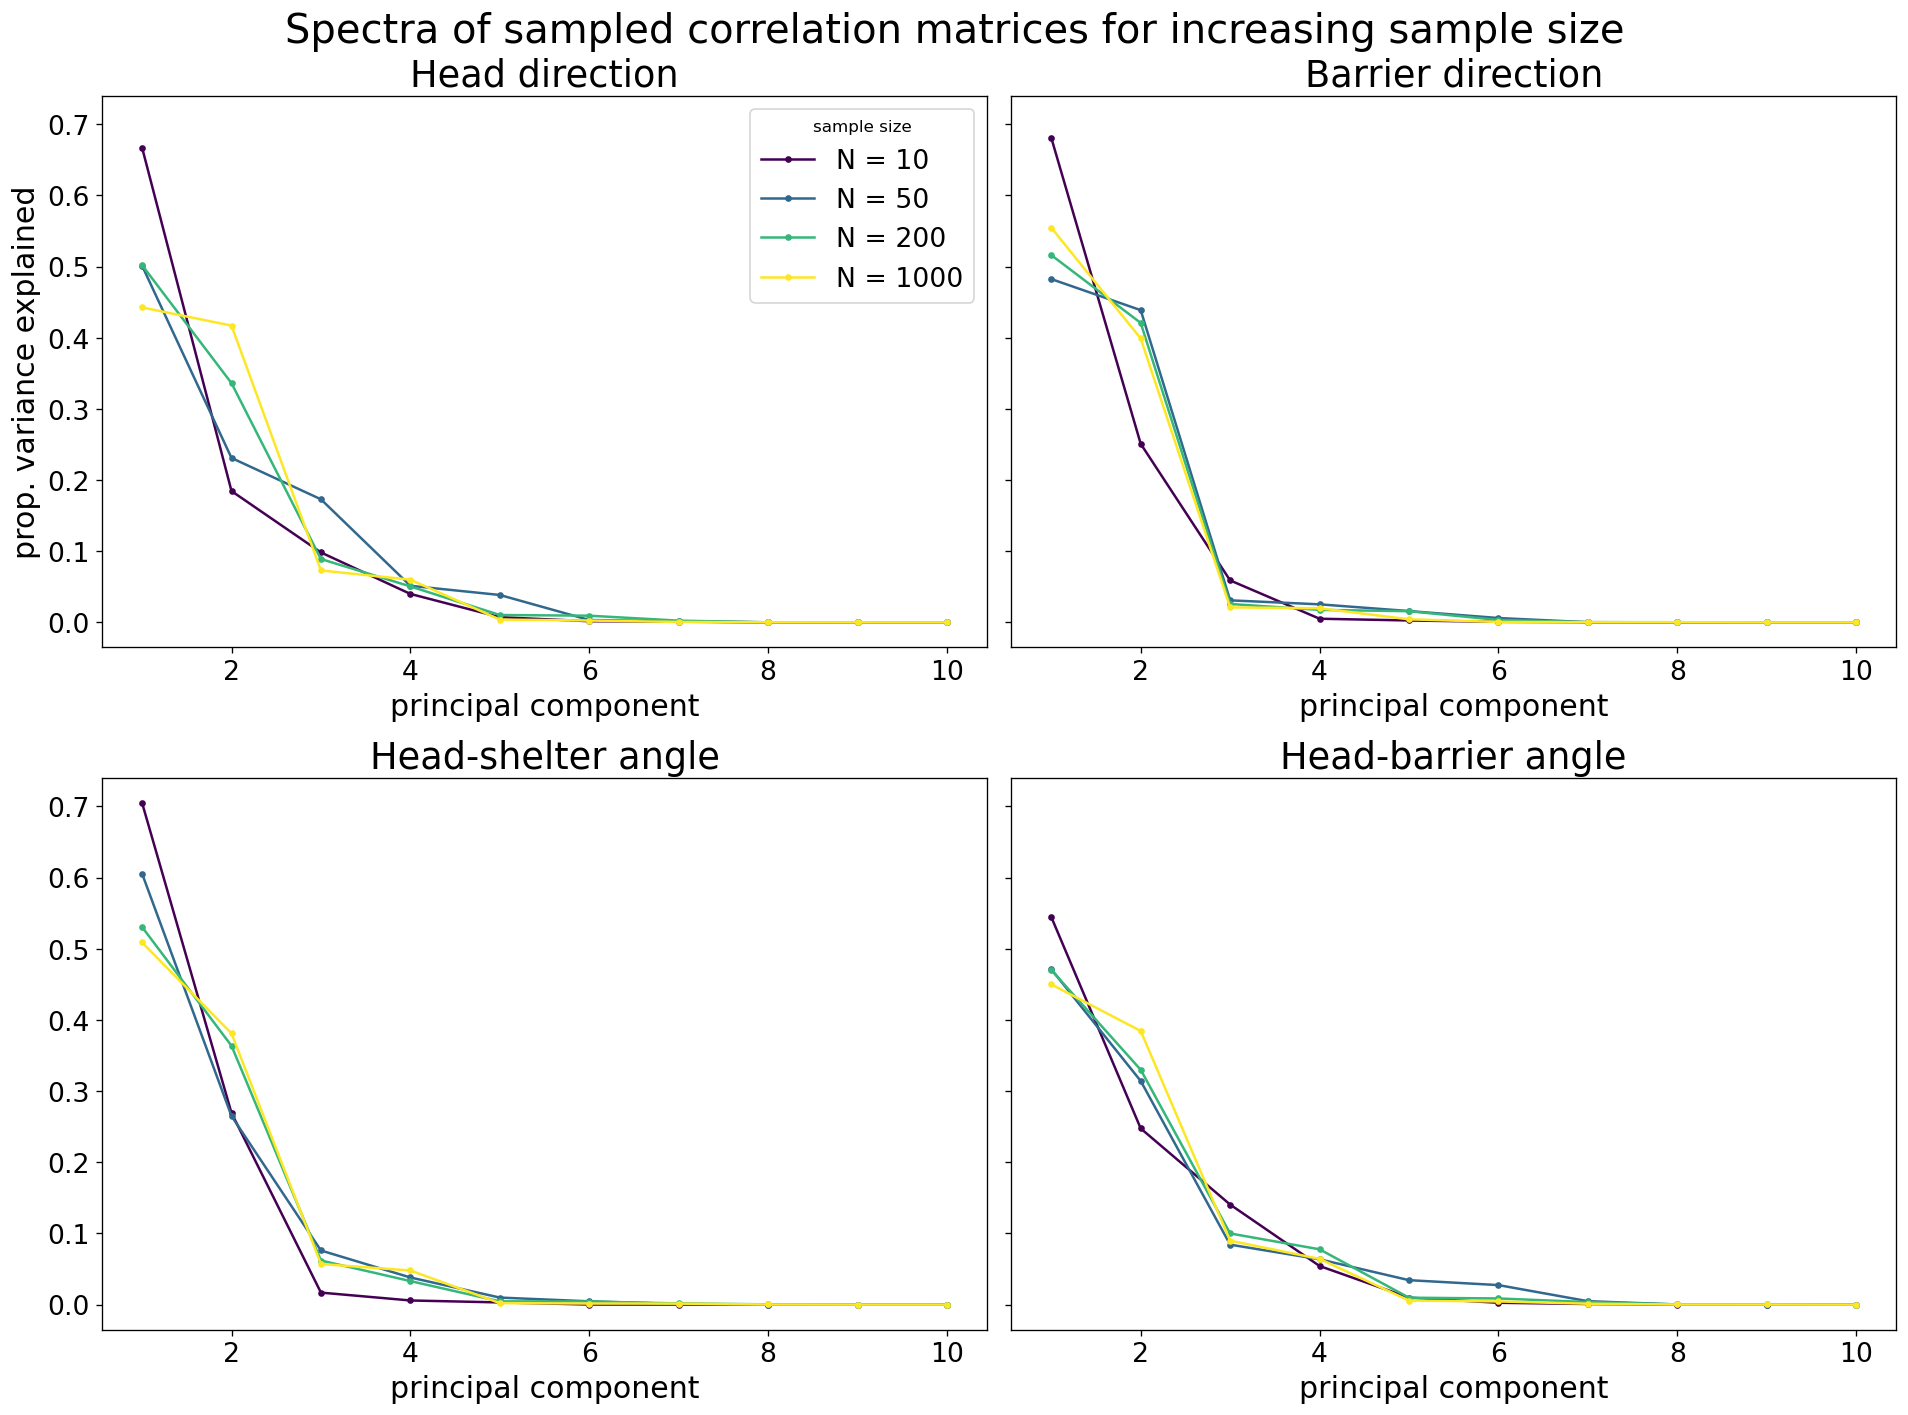
\includegraphics[width=0.9\textwidth]{presentation_figures/item9b_corr_svals.png}
\end{frame}

\begin{frame}
    \centering
    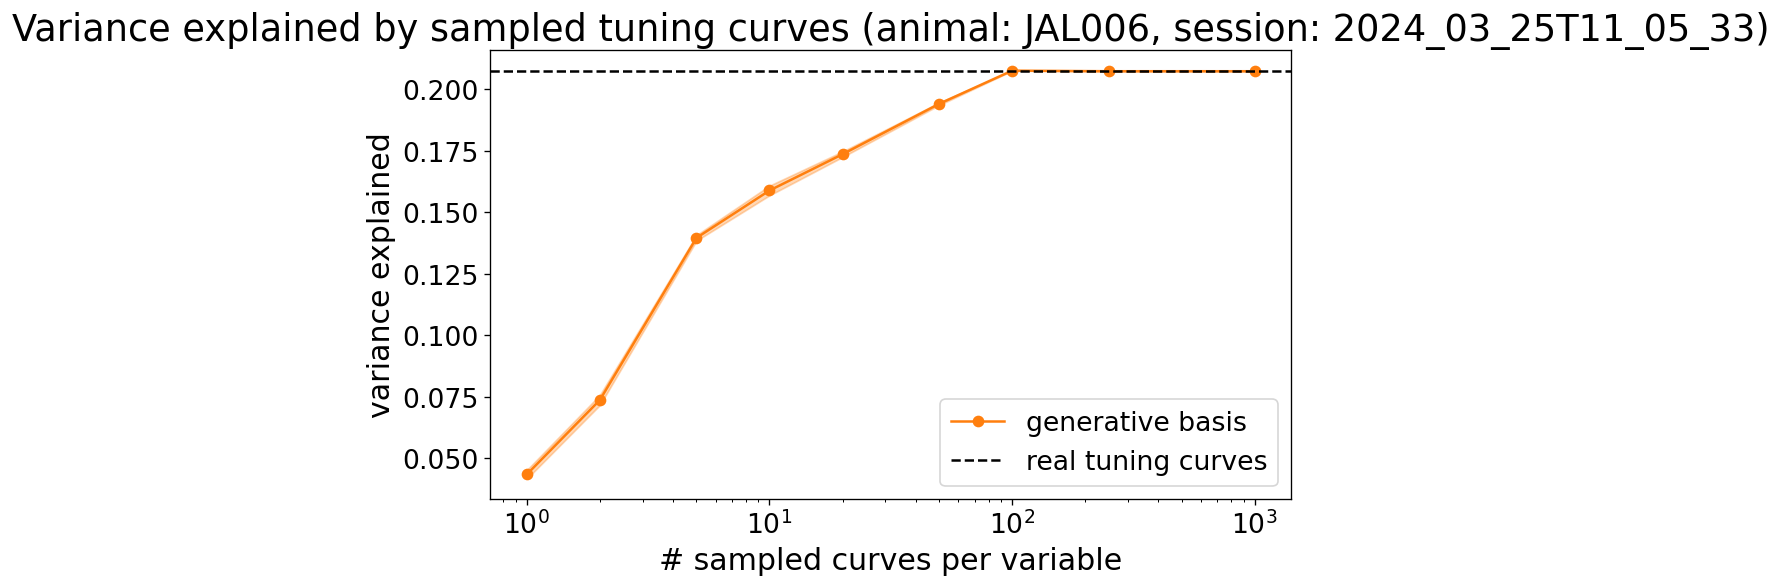
\includegraphics[width=0.9\textwidth]{presentation_figures/item10_generative_ve.png}
\end{frame}

\begin{frame}{Tuning Analysis: Generative Model}
    What does this tell us?

    \begin{itemize}
        \item Observed tunings can be modelled as a finite sample from the generative process.
        \item This generative process is well-behaved as network/sample size increases:
        \begin{itemize}
            \item correlation matrices converge to something reasonable.
            \item variance of overall network captured does not exceed empirical curves.
        \end{itemize}
    \end{itemize}

    There is theory for this: we can describe our finite sample as a projection of the 'true' continuous attractor network:

    \begin{align*}
        \frac{d}{dt} \tilde m(\theta, t) = - \tilde m(\theta, t) + G_{Q(t)} \left(
            \int_{-\pi}^{\pi} \mathcal{J}(\theta - \theta') \tilde m(\theta, t) d \theta'
        \right)
    \end{align*}
    
\end{frame}

\begin{frame}{Tuning Analysis: Mixed Tuning}

    But this was all about 4 separate continuous attractors \dots

    Indeed, the canonical model of coordinate transformations using continuous attractors requires neurons tuned to combinations of both variables.

    \bigskip

    We can play the same game for joint tuning (here focusing on tuning to barrier direction and head-barrier angle)
    
\end{frame}


\begin{frame}
    \centering
    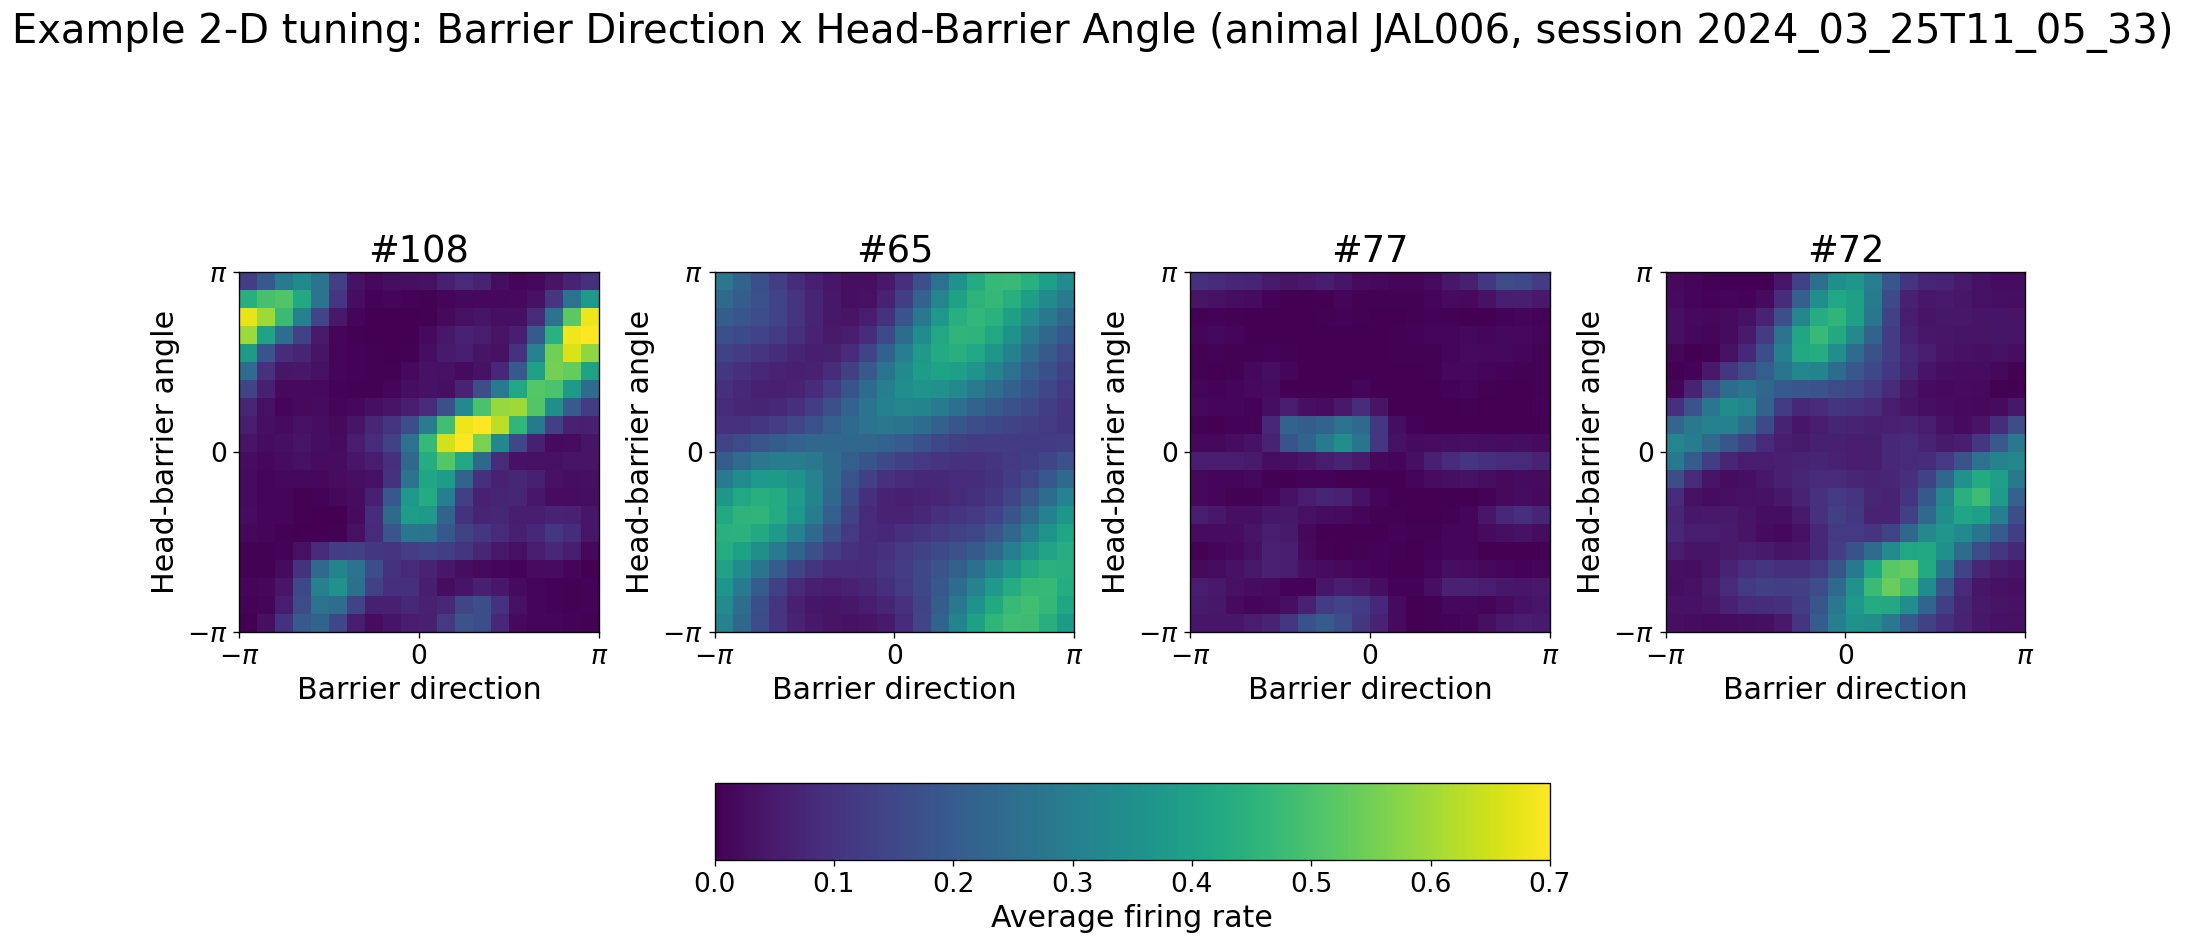
\includegraphics[width=0.9\textwidth]{presentation_figures/item4_tuning2d.png}\
    \vfill
    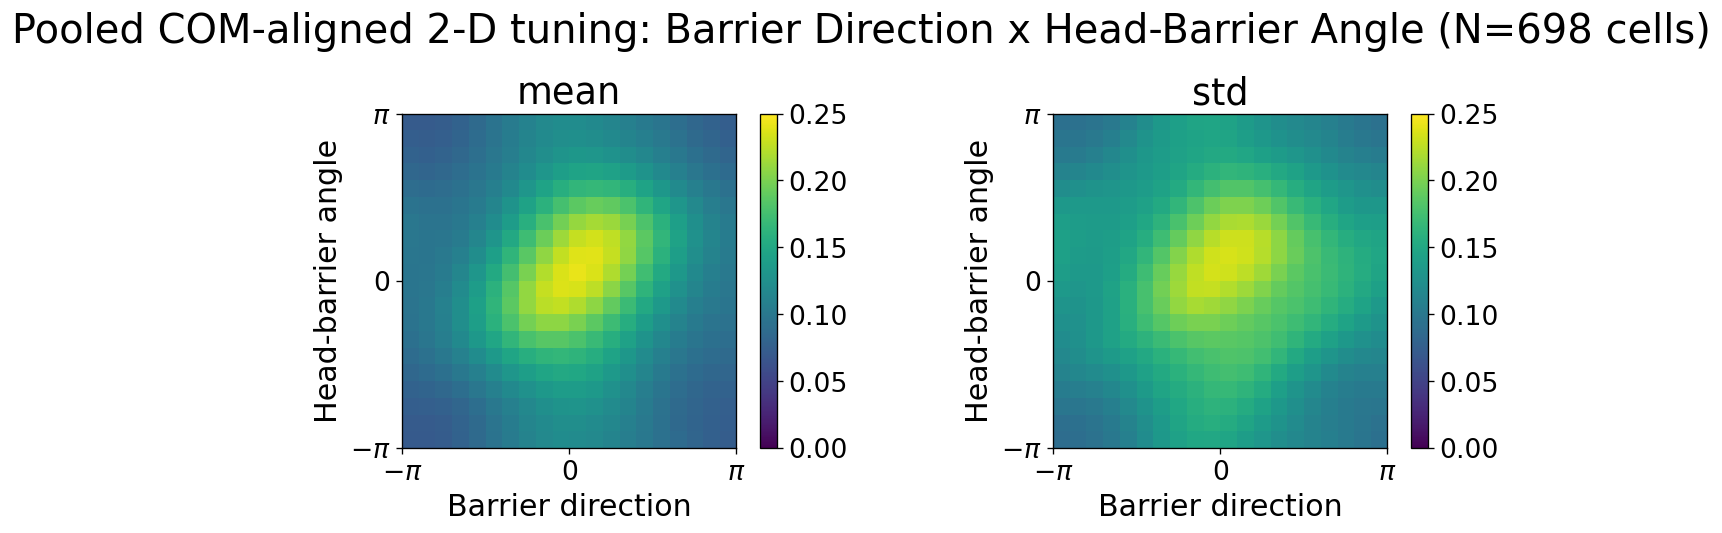
\includegraphics[width=0.8\textwidth]{presentation_figures/item5_pooled2d.png}
    \vfill
\end{frame}

\begin{frame}
    \centering
    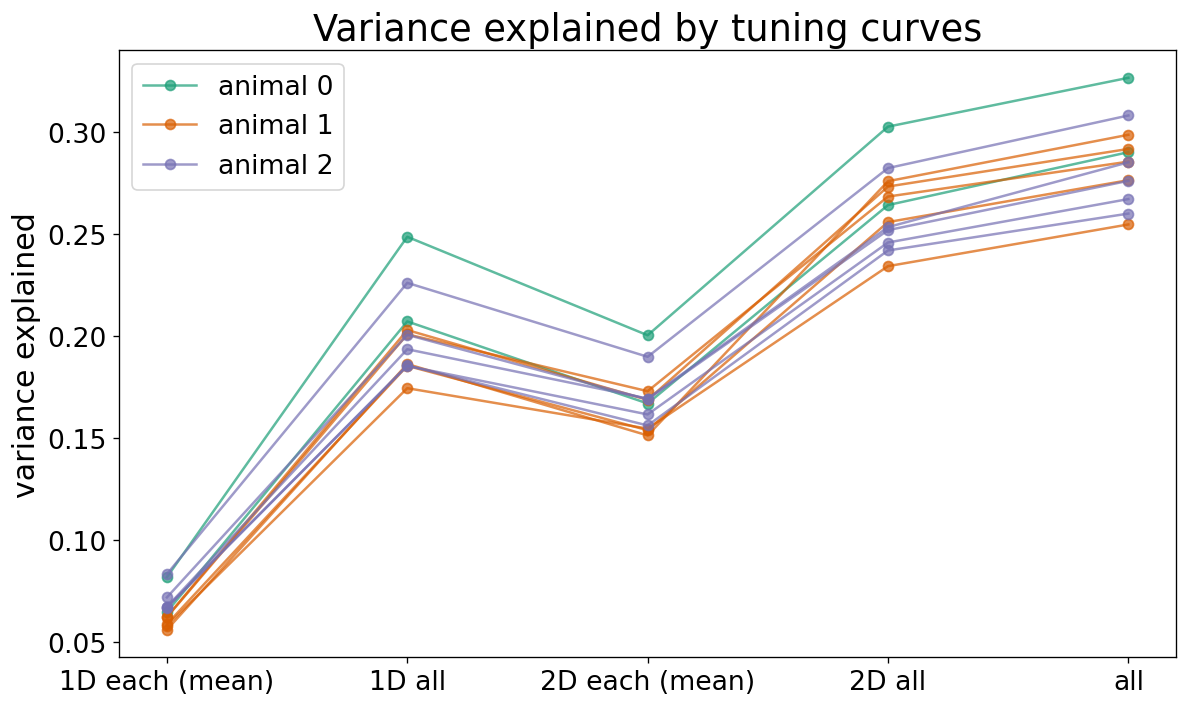
\includegraphics[width=0.9\textwidth]{presentation_figures/item6_regression_ve.png}
\end{frame}


\begin{frame}{Tuning Analysis: Mixed Tuning}

    What does this tell us?

    \begin{itemize}
        \item 2D tuning curves exhibit the same heterogeneity as the 1D curves.
        \item 2D curves explain more variance in the whole network than the 1D curves.
    \end{itemize}

    This would seem to be a promising case study of a neural circuit implementing the classical coordinate transformation circuitry (albeit with disordered embeddings) \dots
    
\end{frame}

\begin{frame}{Tuning Analysis: Barrier Flip}
    \dots but this is not the whole story.

    \medskip

    So far we have not considered the effect of the barrier flip of tuning profiles.

    In the following, we separate sessions into the pre- and post-flip periods and compute tuning curves there separately.
\end{frame}

\begin{frame}
    \centering
    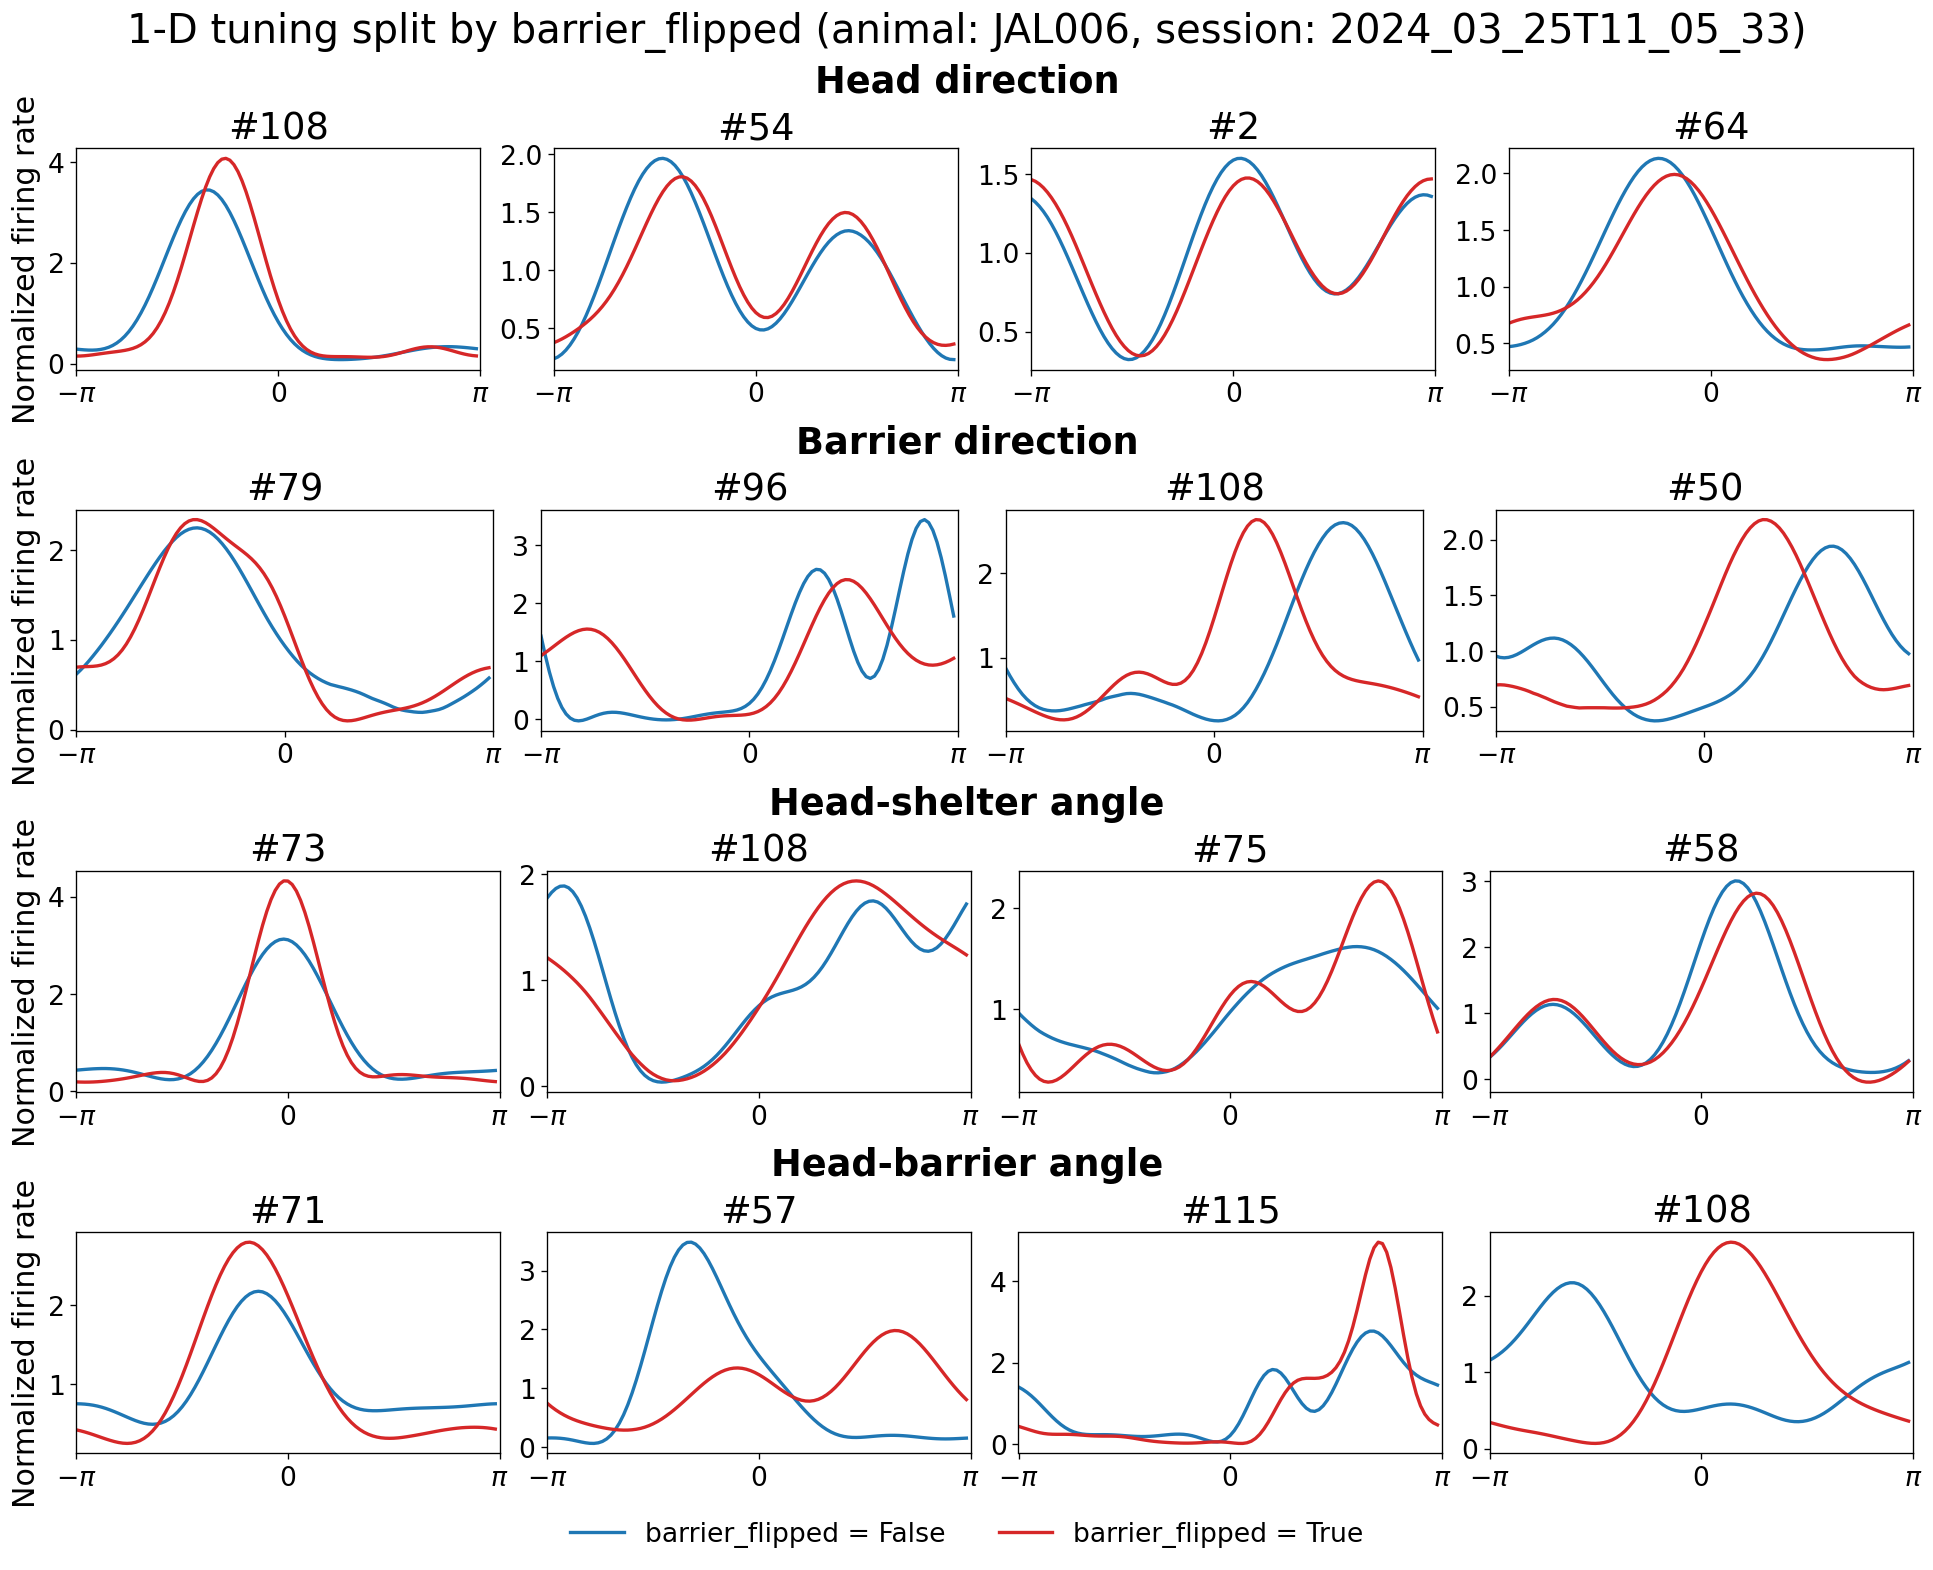
\includegraphics[width=0.9\textwidth]{presentation_figures/item11_barrier_split.png}
\end{frame}

\begin{frame}
    \centering
    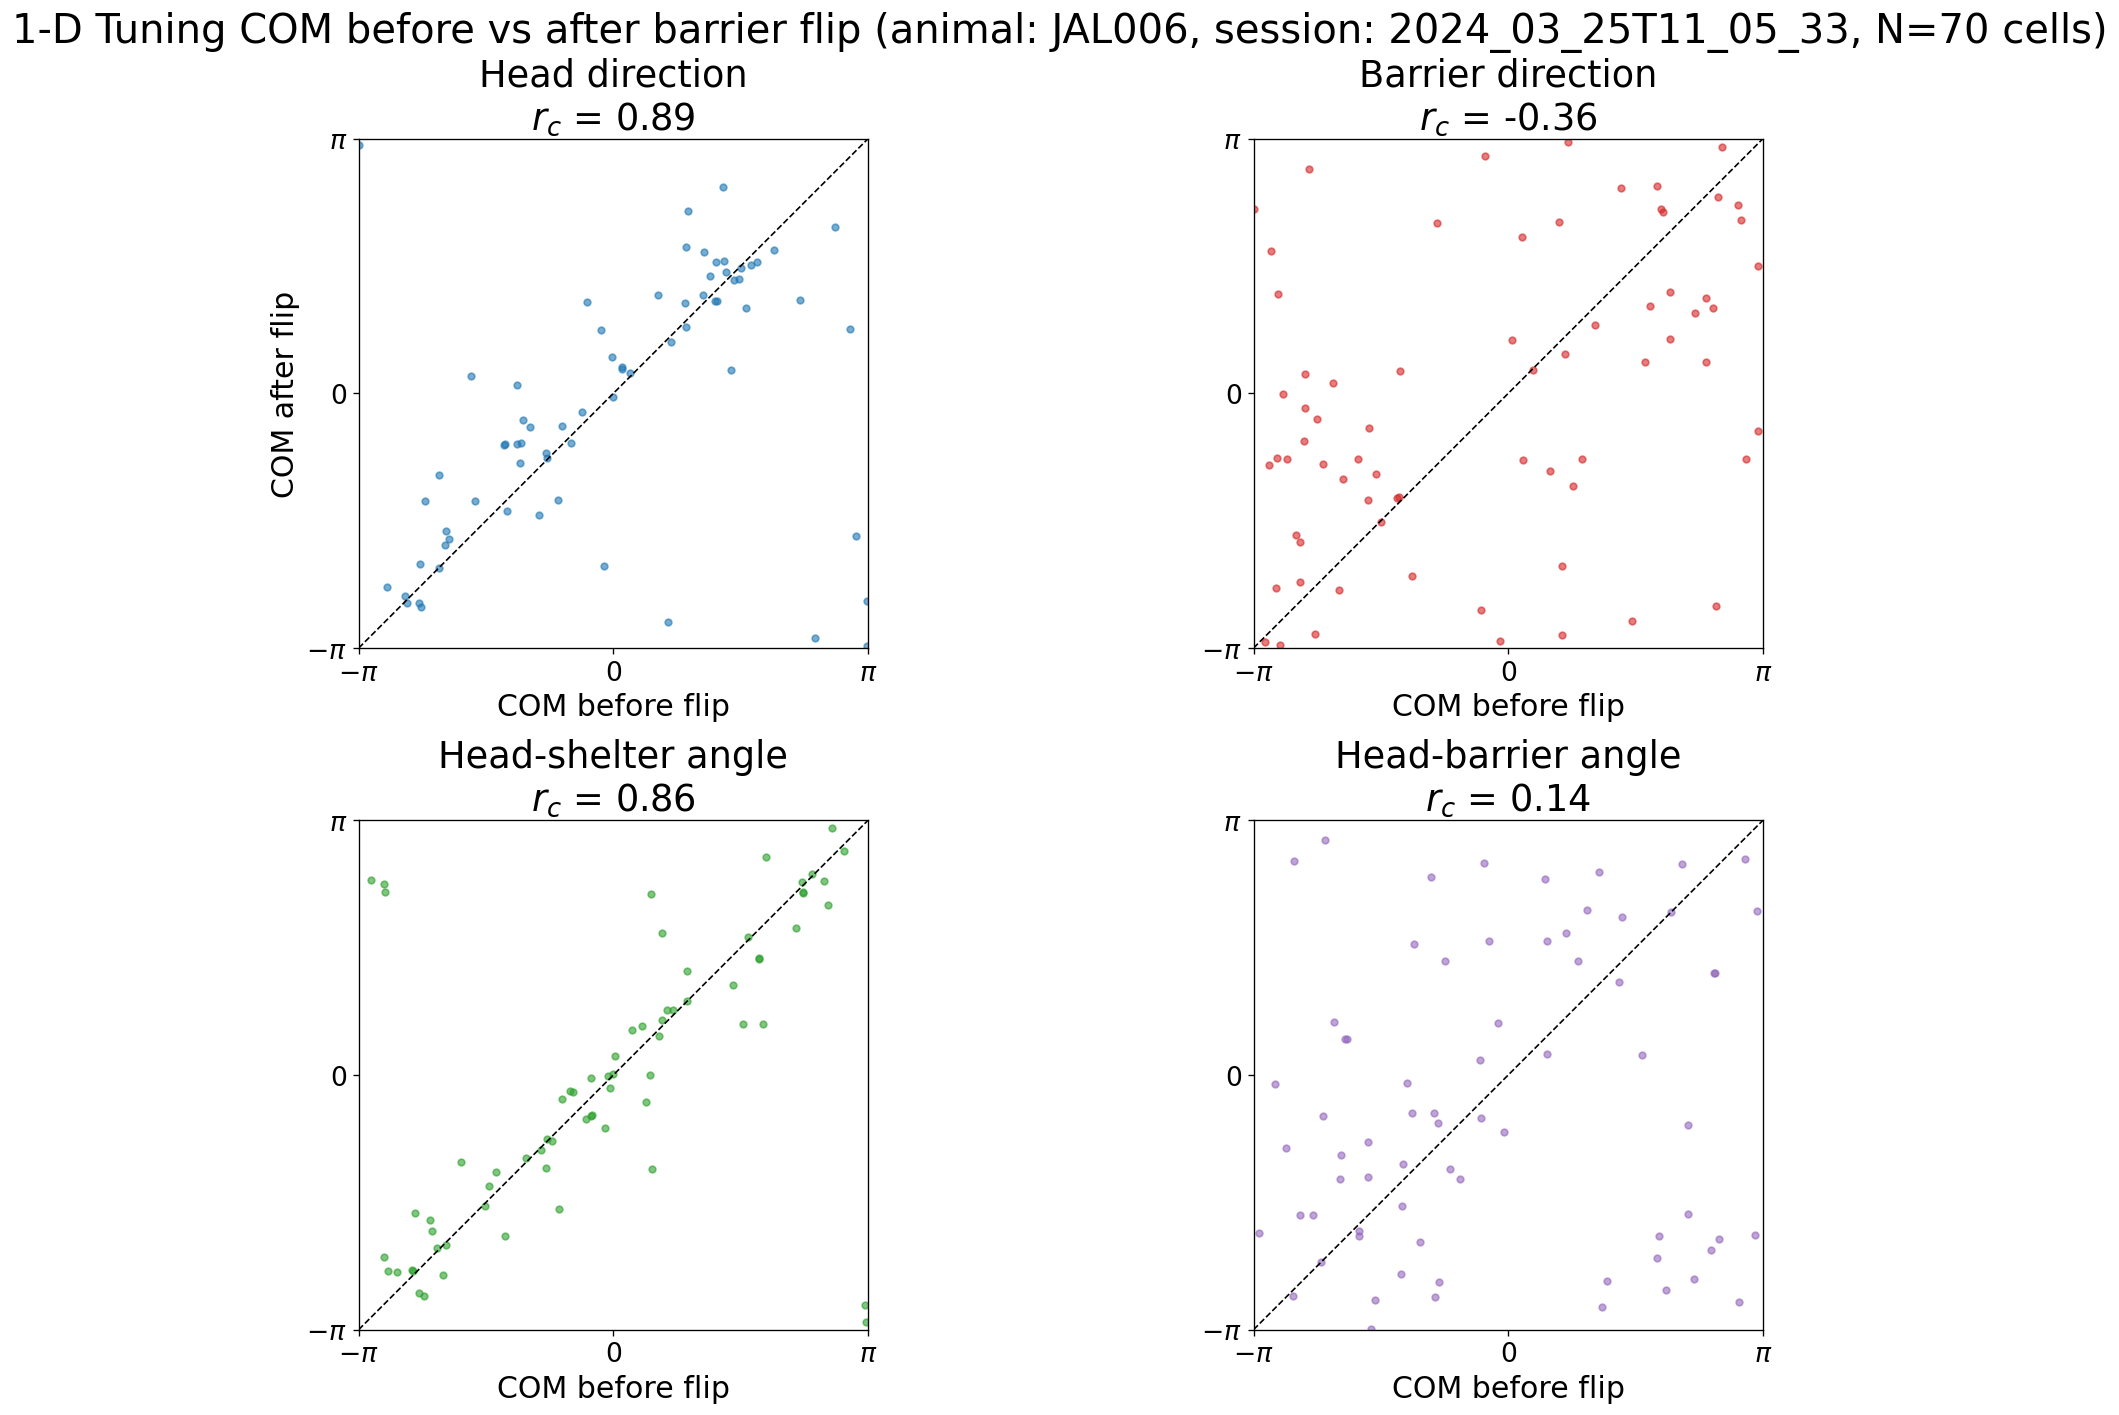
\includegraphics[width=0.9\textwidth]{presentation_figures/item12_barrier_com_corr.png}
\end{frame}

\begin{frame}
    What does this suggest?

    \begin{itemize}
        \item The canonical model of coordinate transformations is really just one big continuous attractor: it may be a good model of variable tracking in a stable environment.
        \item How continuous attractors are used to compute \emph{new} quantities in a changing environment remains an open question.
        \begin{itemize}
            \item e.g., feed-forward models
        \end{itemize}
    \end{itemize}
\end{frame}

{
\setbeamertemplate{navigation symbols}{}
\begin{frame}[plain]
    \centering
    \vfill

    {\usebeamerfont{title}\usebeamercolor[fg]{title}
    \Huge Modelling\par}

    \vspace{0.8em}

    {\usebeamerfont{subtitle}\usebeamercolor[fg]{subtitle}
    \Large Do continuous attractors arise in RNNs?\par}

    \vfill
\end{frame}
}

\begin{frame}{Modelling}

    Do continuous attractors arise in task-trained RNNs?

    \begin{center}
        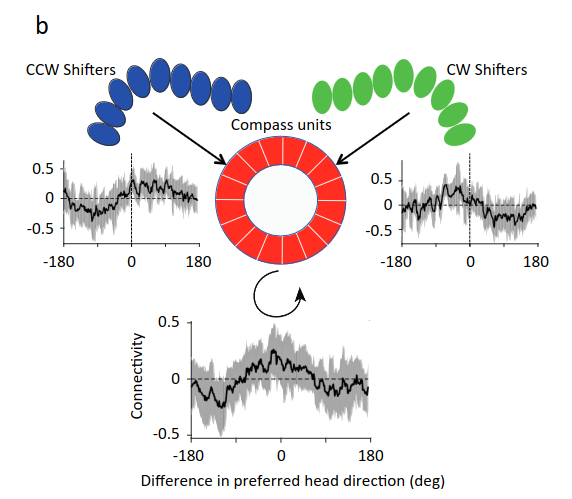
\includegraphics[width=0.5\textwidth]{presentation_figures/cueva_et_al_2020_f3.png}
        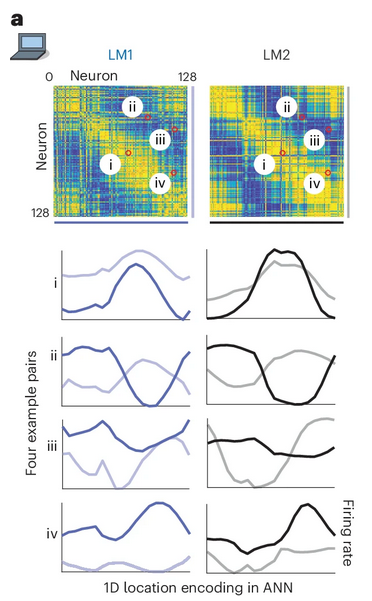
\includegraphics[width=0.3\textwidth]{presentation_figures/voigts_et_al_2025_f3.png}
    \end{center}

    \figsource{\cite{cueva2020}; \cite{voigts2025}}
    
\end{frame}

\begin{frame}{Modelling}
    From our modelling (results not shown):

    \begin{itemize}
        \item<1-> Continuous attractors do arise in certain tasks \dots
        \item<2-> but RNNs seem to favour low-rank solutions \dots
        \item<3-> and which solutions are favoured is dependent on task construction.
    \end{itemize}
\end{frame}

{
\setbeamertemplate{navigation symbols}{}
\begin{frame}[plain]
    \centering
    \vfill

    {\usebeamerfont{(title)}\usebeamercolor[fg]{title}
    \Huge (Some) Theory\par}

    \vspace{0.8em}


    \vfill
\end{frame}
}


\begin{frame}{Theory}

    The theory for constructing continuous attractors hinges on a few components:

    \begin{itemize}
        \item<1-> Recurrent network
        \item<2-> Symmetric connectivity
        \item<3-> Non-linearity
    \end{itemize}

    \uncover<4->{
        Some ideas I'd like to get floating around:
    }

    \begin{itemize}
        \item<5-> Symmetry
        \item<6-> Topology
        \item<7-> Disorder
        \item<8-> Geometry
        \item<9-> Low-rankness
    \end{itemize}
    
\end{frame}


\begin{frame}{Example: Line Attractor}
    
    We model a neural circuit with a linear dynamical system:

    \begin{equation*}
        \frac{d}{dt} r_i(t) = \sum_j^N A_{ij} r_j(t) + h_i(t)
    \end{equation*}

    or in matrix notation:

    \begin{equation*}
        \frac{d}{dt} r(t) = A r(t) + h(t)
    \end{equation*}

    For a linear system, the relevant directions are given by the \emph{eigenvectors} of $A \rightarrow V \Lambda V^T$. 

    \begin{align*}
        \frac{d}{dt} r     &= V \Lambda V^T r + h\\
        \frac{d}{dt} V^T r &= \Lambda V^T r + V^T h\\
        \frac{d}{dt} \tilde r &= \Lambda \tilde r + \tilde h, \quad \tilde r \doteq V^T r \text{ and } \tilde h \doteq V^T h
    \end{align*}

\end{frame}

\begin{frame}
    Solving in component notation gives:

    \begin{align*}
        \frac{d}{dt} \tilde r_i(t) &= \lambda_i \tilde r_i(t) + \tilde h_i(t)\\
        \implies \tilde r_i(t)     &= \int_0^t \tilde h_i(s) e^{\lambda_i (t-s)}ds
    \end{align*}

    \pause If $\lambda_i = 0$, then $\tilde r_i(t) = \int_0^t \tilde h_i(s) ds$ (i.e. circuit integrates inputs).

    \pause Additionally, if $h(t) = 0$, then $\tilde r(t)$ is a fixed point.

    \pause But there is a whole line of possible $\tilde r_i$: anywhere along the corresponding eigenvector will be a fixed point.

    \pause If all other eigenvalues are $<0$, then all patterns decay to this line.
    
    \pause Thus, we have a \emph{manifold} of fixed points: a line attractor.

    \pause What do we learn?
    \begin{itemize}
        \item<1-> Eigenvalues: if $\lambda_i < 0$, the pattern $\tilde r_i$ dies; if $\lambda_i > 0$, the pattern $\tilde r_i$ runs away; if $\lambda_i = 0$, the pattern is stable.
        \item<2-> Symmetry: the decomposition $A = V \Lambda V^T$ is only guaranteed if $A$ is tranpose-symmetric.
        \item<3-> Updates: by giving inputs along the eigenvectors, $\tilde h$, we can integrate them to maintain the signal.
    \end{itemize}
\end{frame}

\begin{frame}{Symmetry and Topology}

    \pause We saw a linear system can keep track of a 1-dimensional scalar with a line attractor,

    \pause What about a circular variable? \pause This is a change in \emph{topology}.

    \pause 
    To handle this, we have to be more particular about the symmetry of the connectivity (and a non-linearity). For example,

    \begin{align*}
        W(i,j) \rightarrow W(i - j)
    \end{align*}

    is a translation symmetric connectivity; if the subtraction is $\mod 2 \pi$, then we have rotational symmetry.

    \pause
    \textbf{Take-away}: A continuous attractor can track a variable of a particular \emph{topology} by exploiting the right \emph{symmetry}.
    
\end{frame}

\begin{frame}{Symmetry and Topology}

    Classical continuous attractors for a circular variable (ring attractors) choose 

    \begin{align*}
        W(i,j) = W(i - j) \propto \cos(\theta_i - \theta_j)
    \end{align*}

    This is an example of an \emph{ordered embedding} of the symmetry. It predicts tuning curves that are identical up to shifts.

    \medskip

    As we saw, this is a problematic prediction.

    \medskip

    We can allow for more diverse tuning curves by using \emph{disordered embeddings}. These relax the symmetry assumption: weights are no longer exactly symmetric, but retain the eigenstructure of symmetric weights.
    
\end{frame}

\begin{frame}{Disorder and Geometry}

    \begin{center}
        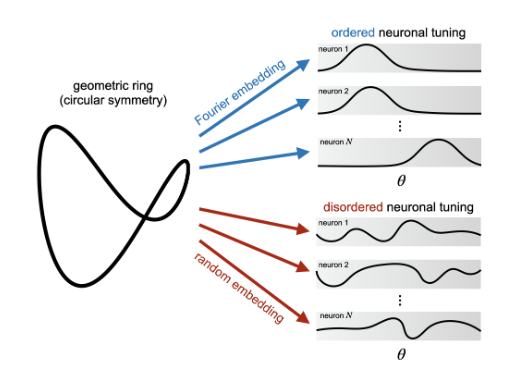
\includegraphics[width=0.75\textwidth]{presentation_figures/clark_et_al_2025_f8.png}
    \end{center}

    \figsource{\cite{clark2025}}

    \textbf{Take-away}: Topology is set by symmetry, or more generally by eigenstructure; \emph{geometry} is determined by the way these symmetries are realised in the network.
    
\end{frame}

\begin{frame}{Disorder and Geometry}

    Large continuous attractor networks with disordered embeddings can be described by an 'effective neural network':

    \begin{align*}
        \frac{d}{dt} \tilde m(\theta, t) = - \tilde m(\theta, t) + G_{Q(t)} \left(
            \int_{-\pi}^{\pi} \mathcal{J}(\theta - \theta') \tilde m(\theta, t) d \theta'
        \right)
    \end{align*}

\end{frame}

\begin{frame}{Disorder and Geometry}

    Some very cool maths behind this! but the rough intuition:

    \begin{itemize}
        \item<1-> As $N \rightarrow \infty$, we can look at \emph{average} quantities rather than individual units
        \begin{itemize}
            \item<2-> A normal CA network labels neurons by their preferred angle: i.e., tracks $x(\theta,t)$
            \item<2-> An effective CA network tracks $m(\theta, t)$: the correlation between the network state at time $t$ and the attractor state for angle $\theta$.
        \end{itemize}
        \item<3-> These averages behave like classical continuous attractor networks, with symmetric interactions: synaptic weights $W(\theta_i - \theta_j)$ are replaced by 'effective interactions' $\mathcal{J}(\theta - \theta')$, the average influence of a $\theta$-tuned state on a $\theta'$-tuned state.
        \item<4-> These interactions have the interesting property that they are modulated by global activity in the network (hence the subscript $Q(t)$).
        \item<5-> Measuring these interactions may allow determining which continuous attractor circuits are connected.
    \end{itemize}
    
\end{frame}

\begin{frame}{2. Functional Connectivity}

    \centering
    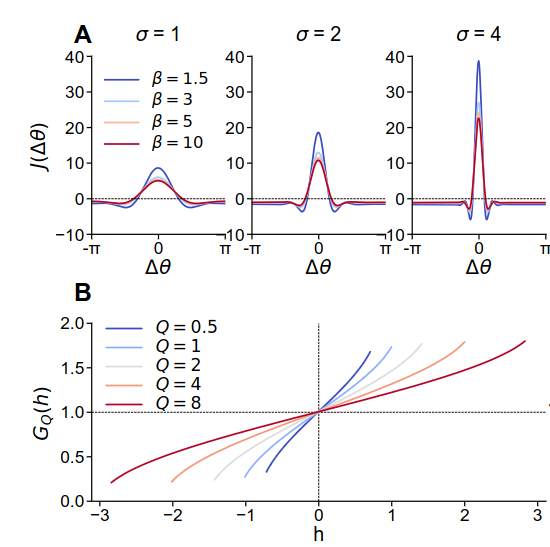
\includegraphics[width=0.7\textwidth]{presentation_figures/clark_et_al_2025_f9.png}

    \figsource{\cite{clark2025}}
\end{frame}

\begin{frame}{Low-Rankness}

    A popular framework for studying recurrent networks uses low-rank connectivity structures \parencite{mastrogiuseppe2018}:

    \begin{align*}
        W_{ij} \propto \sum_r^R m_i^{(r)} n_j^{(r)}
    \end{align*}

    For a rank $R$ connectivity, we can express the state of the network in terms of just $R$ 'latent' variables.

    \centering
    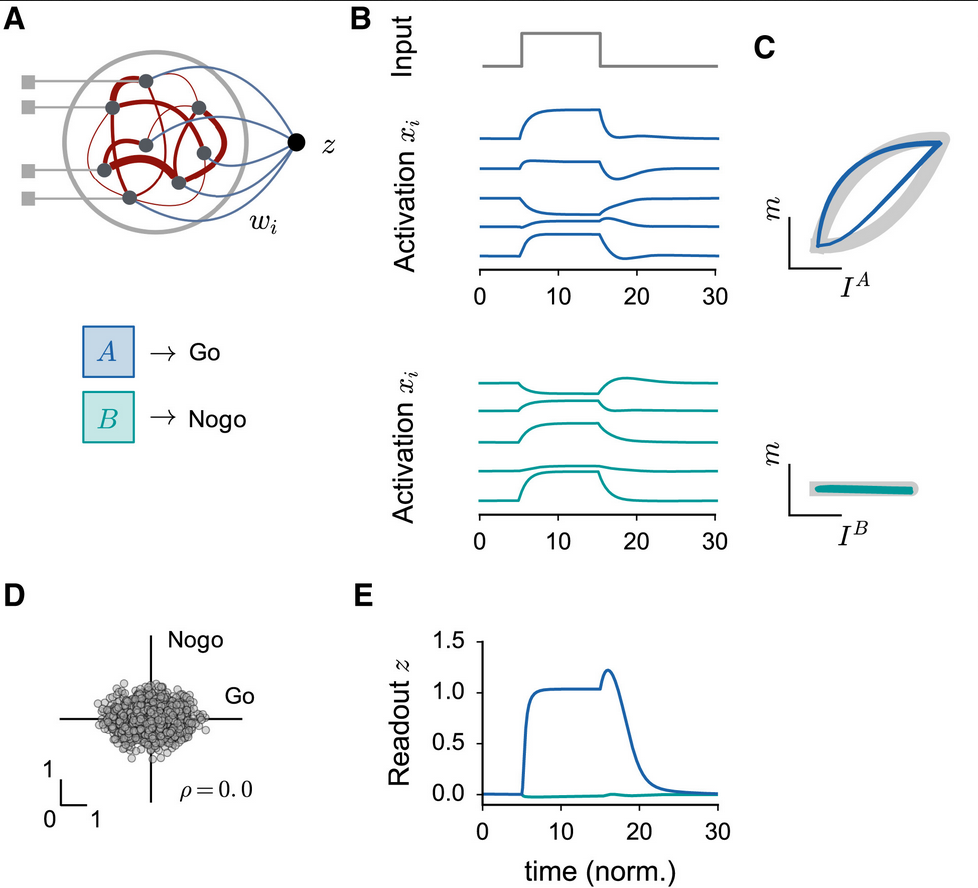
\includegraphics[width=0.4\textwidth]{presentation_figures/mastro_ostojic_2018_f3.png}

    \figsource{\cite{mastrogiuseppe2018}}
\end{frame}

\begin{frame}{Low-Rankness}

    Consider the connectivity:

    \begin{align*}
        W(i,j) = \cos(\theta_i - \theta_j) = \cos(\theta_i) \cos(\theta_j) + \sin(\theta_i) \sin(\theta_j)
    \end{align*}

    This is a low-rank network! It has rank $R=2$ with

    \begin{align*}
        m^{(1)}_i = n^{(1)}_i &= \cos(\theta_i) \\
        m^{(2)}_i = n^{(2)}_i &= \sin(\theta_i)
    \end{align*}

    Thus the network state lies in two dimensions: $\sin\theta(t)$ and $\cos\theta(t)$
    
\end{frame}

\begin{frame}{Low-Rankness}

    But we could equally choose (while still preserving rotational symmetry):

    \begin{align*}
        W(i,j) &= \cos(\theta_i - \theta_j) + \cos(2(\theta_i - \theta_j)) \\
        &= \cos(\theta_i) \cos(\theta_j) + \sin(\theta_i) \sin(\theta_j) \\
        & \quad + \cos(2 \theta_i) \cos(2 \theta_j) + \sin(2 \theta_i) \sin(2\theta_j)
    \end{align*}

    This has rank $R=4$ and the network state lies in four dimensions: $\sin\theta(t)$, $\cos\theta(t)$, $\sin 2\theta(t)$, and $\cos 2\theta(t)$.

    \textbf{Take-away}: We can construct increasingly complicated tuning curves with networks of increasing rank.
    
\end{frame}

\begin{frame}{Theory}
    \centering
    \resizebox{0.95\textwidth}{!}{%
        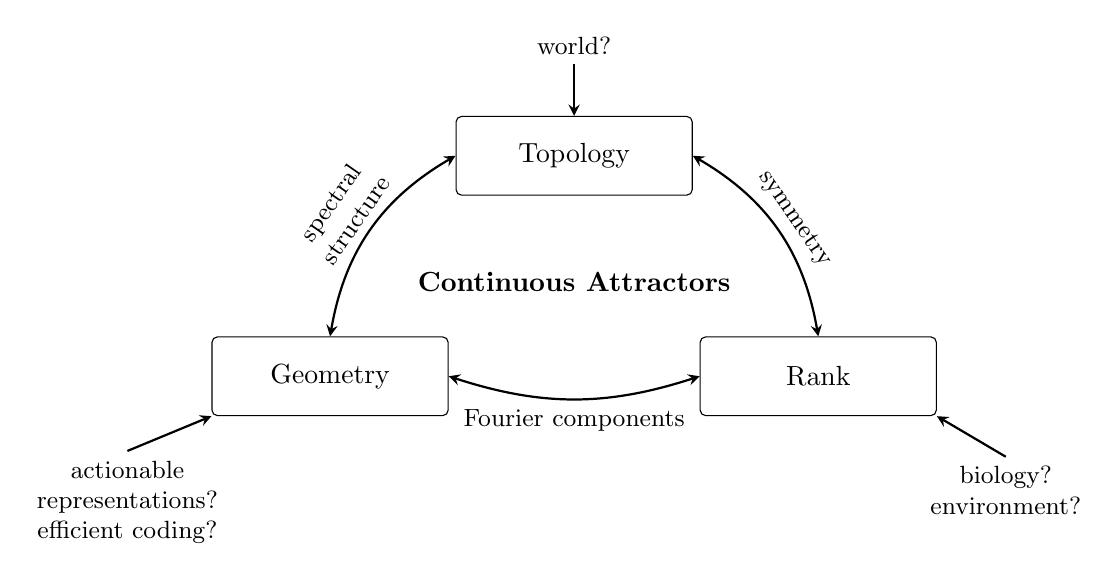
\begin{tikzpicture}[
            box/.style={draw, rounded corners=2pt,
                        minimum width=3.0cm, minimum height=1.0cm, align=center},
            arr/.style={->, thick, >=stealth},
            lab/.style={font=\small, align=center}
        ]

        % Nodes
        \node[box] (topology) at (0,2.1) {Topology};
        \node[box] (geometry) at (-3.1,-0.7) {Geometry};
        \node[box] (rank) at (3.1,-0.7) {Rank};

        % World arrow
        \node[lab] (world) at (0,3.5) {world?};
        \draw[arr] (world) -- (topology);

        % Topology to geometry/rank
        \draw[<->, thick, >=stealth, bend right=25]
            (topology.west) to node[lab, above, sloped] {spectral\\structure} (geometry.north);

        \draw[<->, thick, >=stealth, bend left=25]
            (topology.east) to node[lab, above, sloped] {symmetry} (rank.north);

        % Geometry to rank: curves downward
        \draw[<->, thick, >=stealth, bend right=18]
            (geometry.east) to node[lab, below] {Fourier components} (rank.west);

        % Central label
        \node[lab,font=\bfseries] at (0,0.5) {Continuous Attractors};

        % Side annotations
        \node[lab, anchor=east] (repr) at (-4.4,-2.3)
            {actionable\\representations?\\efficient coding?};

        \draw[arr] (repr.north) -- (geometry.south west);

        \node[lab, anchor=west] (bio) at (4.4,-2.15)
            {biology?\\environment?};

        \draw[arr] (bio.north) -- (rank.south east);

        \end{tikzpicture}%
    }
\end{frame}

{
\setbeamertemplate{navigation symbols}{}
\begin{frame}[plain]
    \centering
    \vfill

    {\usebeamerfont{title}\usebeamercolor[fg]{title}
    \Huge Next steps\par}

    \vspace{0.8em}

    {\usebeamerfont{subtitle}\usebeamercolor[fg]{subtitle}
    \Large What to do?\par}

    \vfill
\end{frame}
}

\begin{frame}
    Following this analysis, I have a few questions:

    \begin{itemize}
        \item<1-> When/why/how do continuous attractors emerge in task-trained RNNs?
        \item<2-> How can we differentiate 'dynamic' computations from 'static' ones? Recurrent from feed-forward? What are the implications for continuous attractor networks?
        \item<3-> How does learning interact with continuous attractors?
    \end{itemize}
\end{frame}

\begin{frame}{1. Theory}

    \begin{itemize}
        \item<1-> When do continuous attractors arise in task-trained RNNs?
        \item<2-> What factors of the task shape the topology/geometry of the attractor?
        \item<3-> Can we leverage this to train biologically relevant models?
    \end{itemize}
    
\end{frame}

\begin{frame}{1. Theory}

    \begin{itemize}
        \item When do continuous attractors arise in task-trained RNNs?
        \item What factors of the task shape the topology/geometry of the attractor?
        \item Can we leverage this to train biologically relevant models?
    \end{itemize}

    \medskip
    An attractive framework: Statistical field theory.
    
\end{frame}

\begin{frame}{2. Functional Connectivity}

    Large continuous attractor networks with disordered embeddings can be described by an 'effective neural network':

    \begin{align*}
        \frac{d}{dt} \tilde m(\theta, t) = - \tilde m(\theta, t) + G_{Q(t)} \left(
            \int_{-\pi}^{\pi} \mathcal{J}(\theta - \theta') \tilde m(\theta, t) d \theta'
        \right)
    \end{align*}

\end{frame}

\begin{frame}{2. Functional Connectivity}

    \centering
    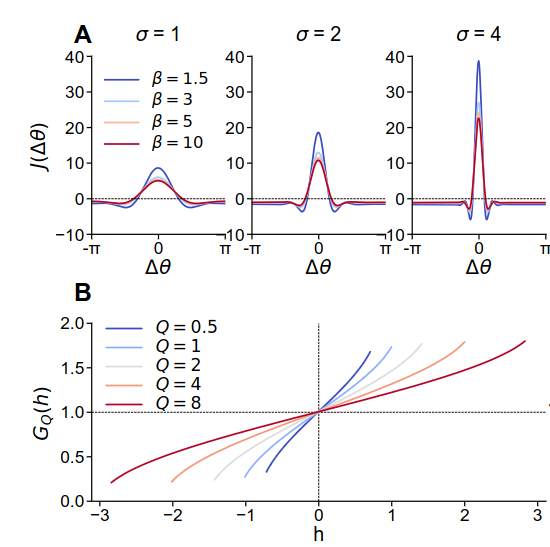
\includegraphics[width=0.7\textwidth]{presentation_figures/clark_et_al_2025_f9.png}

    \figsource{\cite{clark2025}}
\end{frame}

\begin{frame}{3. Learning Dynamics}
    
    Low-rank recurrent networks are particularly amenable to analysis of learning dynamics (under gradient descent \dots )

    \medskip

    Activity in low-rank networks is determined by the alignment between weight vectors (overlaps).

    Recent work \parencite{ger2026} has shown that, when training under gradient descent, some of these overlaps are 'loss-visible' and some are 'loss-invisible'.

    \medskip

    They also showed that these loss-invisible overlaps can contribute to hysteretic effects in learning trajectories.

\end{frame}

\begin{frame}{3. Learning Dynamics}

    Suppose you have a rank-1 linear network that receives a scalar input $h(t)$ and produces a scalar output $y(t)$:

    \begin{align*}
        \frac{d}{dt} x(t) &= -x(t) + \frac{1}{N} m n^T x(t) + u h(t) \\
        y(t) &= v^T x(t)
    \end{align*}

    The connectivity vectors are $(m, n, u, v)$

    We can write this in latent-space as:

    \begin{align*}
        \frac{d}{dt} \kappa(t) = - \kappa(t) + \begin{bmatrix}
            0 & 0 \\ \frac{1}{N} n^T u & \frac{1}{N} n^T m
        \end{bmatrix} \kappa(t) + \begin{bmatrix}
            1 \\ 0
        \end{bmatrix} x(t) 
    \end{align*}

    \begin{align*}
        y(t) = \begin{bmatrix}
            \frac{1}{N} v^T u & \frac{1}{N} v^T m
        \end{bmatrix} \kappa(t)
    \end{align*}

    The overlaps that matter to the dynamics are $(n \cdot u, n \cdot m, v \cdot u, v \cdot m)$. 
    
    But there are other overlaps! For example $u \cdot m$.

    These are the loss-visible and loss-invisible overlaps.
    
\end{frame}

\begin{frame}
    
    \centering
    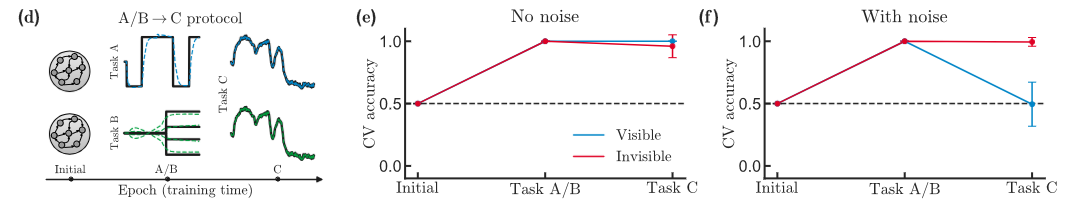
\includegraphics[width=0.95\textwidth]{presentation_figures/ger_barak_2026_f4.png}

    \figsource{\cite{ger2026}}
\end{frame}

\begin{frame}{Conclusions}

    \begin{itemize}
        \item<1-> Continuous attractors appear a good model of ($\approx$ 30 \% of) retrosplenial cortex in a static environment.
        \item<2-> We can interrogate this by looking at the functional connectivity between cells and comparing it to theory.
        \item<3-> The classical models appear to fail when the environment changes: the classical coordinate transformation circuitry may be a better model of 'error correction' than bona fide computation.
        \item<4-> This leaves a few lines of study:
        \begin{itemize}
            \item<5-> How can we mesh the task-trained RNN literature with biological continuous attractors? What can we learn from the fact that they do not naively converge to the same attractors?
            \item<6-> How does the continuous attractor picture change when 'dynamic' computation is involved? How can we discern the 'static' from a 'dynamic' model of coordinate transformation?
            \item<7-> Can we use low-rank networks and continuous attractors to model learning dynamics in natural settings?
        \end{itemize}
    \end{itemize}

\end{frame}

\nocite{*}
\begin{frame}[allowframebreaks]{References}
    \tiny
    \printbibliography[heading=none]
\end{frame}


\end{document}